% MURU-BENCH: A Benchmark for Mathematical Reasoning Under Uncertainty
% NeurIPS 2026 Datasets and Benchmarks Track

\documentclass{article}

% NeurIPS style
\usepackage[final]{neurips_2024}

\usepackage[utf8]{inputenc}
\usepackage[T1]{fontenc}
\usepackage{hyperref}
\usepackage{url}
\usepackage{booktabs}
\usepackage{amsfonts}
\usepackage{amsmath}
\usepackage{amssymb}
\usepackage{nicefrac}
\usepackage{microtype}
\usepackage{graphicx}
\usepackage{xcolor}
\usepackage{subcaption}
\usepackage{algorithm}
\usepackage{algorithmic}
\usepackage{multirow}
\usepackage{enumitem}
\usepackage{wrapfig}
\usepackage{pifont}
\usepackage{amsthm}

\emergencystretch=3em

\newcommand{\muru}{\textsc{Muru-Bench}}
\newcommand{\ci}{\mathrm{CI}}
\newcommand{\ece}{\mathrm{ECE}}

\title{MURU-BENCH: A Benchmark for Mathematical Reasoning Under Uncertainty}

\author{
  Swetank Kumar \\
  Department of Computer Science \\
  SRM Institute of Science and Technology (SRMIST) \\
  Chennai, Tamil Nadu, India \\
  \texttt{swetankkumar391@gmail.com} \\
  \url{https://github.com/swetank18}
}

\begin{document}

\maketitle

\begin{abstract}
Mathematical-reasoning benchmarks score correctness as a single number, but the mathematics that matters in practice---epidemiology, reliability engineering, decision support---is uncertain by construction. A benchmark that ignores stated confidence cannot distinguish a calibrated reasoner from a confident guesser. We introduce \muru{} (\textbf{M}athematical \textbf{R}easoning \textbf{U}nder \textbf{U}ncertainty \textbf{Bench}mark), a 3{,}000-problem benchmark where every prediction is scored on four orthogonal dimensions: point estimate, confidence-interval coverage, stated-confidence calibration, and reasoning-framework identification. Problems span five categories---Bayesian Updating, Conditional Probability Chains, Distribution Estimation, Decision Under Uncertainty, and Adversarial Ambiguity---and five difficulty levels, generated by 21 parametric templates with closed-form solutions, so correctness is guaranteed by construction and the dataset is reseedable to arbitrary scale. The harness reports six metrics including Expected Calibration Error and a safety-relevant overconfidence rate, and ships a unified API client for six hosting providers.

We first validate the harness with five simulated capability tiers: paired McNemar tests detect every adjacent-tier gap at $p < 10^{-3}$, including the smallest configured gap of 11.6 percentage points, establishing that the 301-problem test split has statistical power to discriminate tier-scale differences. We then report the first language-model leaderboard on \muru{}, evaluating five hosted open-weights models. Headline Accuracy@CI spans 53 percentage points (Llama-3.1-8B: 43.9\%; GPT-OSS-120B: 97.0\%). Across the panel, accuracy and calibration in level are \emph{separable}: the rank correlation between Accuracy@CI and ECE is $\rho = -0.10$ (exact $p = 0.95$; $n = 5$ models), and the second-most-accurate model is the fourth-best calibrated. The metrics that do track accuracy perfectly---the overconfidence rate and the Brier score, both $\rho = -1.00$---are functions of the error rate rather than of calibration shape, a distinction a benchmark has to report enough metrics to make. Calibration in level is not metacognition either: under a Murphy decomposition every model has resolution $\leq 0.012$ against outcome uncertainties up to $0.246$, and AUROC of stated confidence over correctness spans $0.439$--$0.575$, with the panel leader \emph{below} chance and the best row only weakly above it---so no model in the panel usefully ranks its own correct answers above its wrong ones, a failure invisible to ECE and to coverage-only metrics, which we surface by adding a proper interval-scoring rule, a Murphy decomposition, and a debiased ECE to the harness. We also report a scoring failure of our own that reviewers of numeric-answer benchmarks should expect to find in theirs: because the prompt asked for ``a single number'' on problems denominated in \$K or in percent, 24.7\% of the panel's recorded errors were correct answers in an admissible unit, and correcting them moves the leaderboard, dissolves an apparent accuracy/calibration coupling ($\rho = -0.90 \to -0.10$), and dissolves an apparent hedging result. Because that correction is applied post hoc, we validate it against a pre-registered prediction: a paired 100-problem re-run under a prompt that states the convention is statistically indistinguishable from the corrected scoring, differs from the uncorrected one, and produces zero unit mismatches, on both panel models whose instruction-following supports the test. Benchmark, harness, raw responses, statistical scripts, and CI are released at \url{https://github.com/swetank18/MURU_proj} under CC-BY-4.0 (data) and MIT (code).
\end{abstract}


\section{Introduction}
\label{sec:introduction}

Recent progress on mathematical benchmarks has been startling. Frontier language models match strong human performance on grade-school word problems~\citep{gsm8k}, hold their own against competition-level mathematics~\citep{math}, and span a wide range of subject areas at adult-expert level~\citep{mmlu}. These benchmarks share a structural feature: each problem has a single deterministic answer. There is no ambiguity in the ground truth, and a response is either right or wrong as a string of characters.

The mathematical reasoning encountered in practice almost never has this shape. A clinician interpreting a diagnostic test combines an uncertain prevalence with imperfect test characteristics. A reliability engineer chains together conditional probabilities estimated from limited data. A policy analyst weighs courses of action against utilities that depend on states whose probabilities are themselves estimated. In each case, the answer is not a number but a distribution or an interval, and the quality of the reasoning depends as much on the stated confidence as on the central estimate.

\paragraph{The calibrated uncertainty gap.}
We argue that the standard evaluation paradigm for language-model mathematics has a load-bearing blind spot: it provides no signal about whether a model knows when it is uncertain. We call this the \emph{calibrated uncertainty gap}. The gap matters operationally, not just academically. A medical-reasoning assistant that returns a confidently incorrect posterior probability is more dangerous than one that flags its own uncertainty. A financial-risk model that reports a point estimate understates tail risk by construction. A policy model that anchors on the most salient figure in a problem stem reproduces the base-rate fallacy at scale. A benchmark that only rewards point accuracy on deterministic problems supplies no metric that can be optimised against these failure modes, because the failure modes are invisible to it.

\paragraph{Contributions.}
This paper makes four contributions.

\begin{enumerate}[leftmargin=*,itemsep=3pt]
    \item A 3{,}000-problem benchmark across five categories of mathematical uncertainty. Each problem ships with a ground-truth point estimate, a confidence interval at a stated level, an ordered list of solution steps, the required reasoning framework, and an enumeration of common failure modes (Section~\ref{sec:dataset}). All 3{,}000 problems are generated by 21 parametric templates with closed-form solutions, so correctness is guaranteed by construction and the benchmark can be expanded by changing the seed.
    \item A four-dimensional evaluation protocol (Section~\ref{sec:formalization}) that scores point accuracy, interval coverage, metacognitive calibration, and framework correctness as orthogonal capabilities, instantiated as six metrics that include Expected Calibration Error and an overconfidence rate (Section~\ref{sec:evaluation}).
    \item A harness-validation study (Section~\ref{sec:results}) using five simulated capability tiers spanning a 70-percentage-point accuracy range. Percentile bootstrap 95\% intervals on every metric ($B = 10{,}000$) and paired McNemar tests on every adjacent-tier comparison establish that the metric implementations recover the intended ordering and that the held-out test split ($n = 301$) has the statistical power to discriminate tier-scale capability differences as small as 11.6 percentage points ($p < 10^{-3}$ throughout).
    \item The first language-model leaderboard on \muru{} (Section~\ref{sec:real_llm}). We report test-split measurements for five hosted open-weights models---Llama-3.1-8B, Llama-3.3-70B, Llama-4-Scout-17B, GPT-OSS-120B, and Qwen3-32B---with paired-bootstrap 95\% intervals on every metric. The leaderboard shows a 53-percentage-point spread in Accuracy@CI on the same problem set, finds accuracy and calibration in level to be separable rather than coupled ($\rho = -0.10$), and surfaces category-shaped weaknesses on Decision-Under-Uncertainty and Adversarial Ambiguity problems that single-number leaderboards on existing benchmarks would not detect. It also reports a scoring correction of our own making---24.7\% of the panel's recorded errors were correct answers in a unit the prompt failed to specify---which is what turned the coupling we expected into the null we report.
\end{enumerate}

\paragraph{Reproducibility and extensibility.}
The harness includes a unified API client for six hosting providers; deterministic generation under a fixed seed; stratified train, validation, and test splits; a 26-test pytest suite that covers metrics, response parsing, and dataset invariants; a continuous-integration configuration that runs the suite on Python 3.10, 3.11, and 3.12 on every push; a Datasheet for Datasets~\citep{gebru2021}; and a Croissant~\citep{croissant2024} metadata file (Appendices~\ref{app:datasheet} and~\ref{app:croissant}). Each row of the leaderboard is reconstructible bit-for-bit from a single per-model JSON archive in \texttt{evaluation/baselines/}, which holds the raw model responses, the parsed predictions, and the computed metrics for every problem in the run.


\section{Related Work}
\label{sec:related}

\paragraph{Mathematical reasoning benchmarks.}
GSM8K~\citep{gsm8k} tests grade-school arithmetic, has a single deterministic answer per problem, and has been largely saturated by frontier models. MATH~\citep{math} extends to competition-level problems across algebra, geometry, and number theory, but each problem still admits a unique numerical or symbolic answer. BIG-Bench Hard~\citep{bigbench} broadens the task distribution but contains no formal probability problems. MathBench~\citep{liu2024} is hierarchical across education levels but does not require uncertainty quantification. TheoremQA~\citep{chen2023} probes theorem application against deterministic targets. None of these benchmarks ask a model to produce a calibrated confidence interval as part of the answer; the ground-truth label is always a single object.

\paragraph{Calibration and confidence in language models.}
\citet{kadavath2022} showed that language models possess a partial, noisy signal of their own correctness through token probabilities. \citet{guo2017} introduced the binned Expected Calibration Error metric we adopt. Prompting strategies for verbalised confidence~\citep{tian2023} elicit confidence values that correlate with accuracy but exhibit systematic biases, particularly overconfidence in long-tail domains. \citet{xiong2024} surveys this literature and finds that scale improves calibration on average without eliminating its failure modes. The connecting thread is that calibration is studied as a property of the model's metacognition over an existing benchmark, rather than as a target the benchmark itself measures. \muru{} differs by promoting calibration to a first-class evaluation target, with ground-truth confidence intervals against which the model's stated confidence can be scored.

\paragraph{Uncertainty quantification.}
The machine-learning literature on predictive uncertainty---Bayesian neural networks~\citep{gal2016}, deep ensembles~\citep{lakshminarayanan2017}, conformal prediction~\citep{angelopoulos2022}---studies how to make a learned model report uncertainty about its own predictions. \muru{} tests something different and prior to that machinery: whether a model can reason about uncertainty as a mathematical concept in the first place. The skill we measure is computing posteriors, propagating parameter uncertainty through compositions, and recognising when a problem admits multiple defensible formalisations.

\paragraph{Adversarial and ambiguous evaluation.}
TruthfulQA~\citep{lin2022} probes whether models repeat popular misconceptions when asked. The Adversarial Ambiguity category in \muru{} is structurally analogous in that it deliberately stresses confident but wrong reasoning. The mechanism is different: TruthfulQA exploits world-knowledge cues, while our adversarial problems are mathematically precise and exploit ambiguity in the formalisation rather than in the facts.

\paragraph{Positioning.}
Table~\ref{tab:comparison} places \muru{} alongside the closest reference benchmarks. To our knowledge, it is the first benchmark that combines formal mathematical reasoning with calibrated uncertainty quantification, requires both correct computation and calibrated confidence, and arranges problems on a structured difficulty hierarchy.

\begin{table}[t]
\centering
\caption{Comparison of \muru{} with existing mathematical-reasoning benchmarks. \muru{} is the only benchmark in this list that requires calibrated confidence intervals as part of the answer, that contains adversarial ambiguity by design, and that scores calibration directly. {\footnotesize\ding{51}} = yes, {\footnotesize\ding{55}} = no, {\footnotesize$\sim$} = partial.}
\label{tab:comparison}
\resizebox{\textwidth}{!}{%
\begin{tabular}{lccccccc}
\toprule
\textbf{Benchmark} & \textbf{Size} & \textbf{Math} & \textbf{Uncertainty} & \textbf{CI Required} & \textbf{Calibration} & \textbf{Adversarial} & \textbf{Difficulty} \\
 & & \textbf{Reasoning} & \textbf{Reasoning} & \textbf{in Answer} & \textbf{Measured} & \textbf{Ambiguity} & \textbf{Levels} \\
\midrule
GSM8K & 8.5K & \ding{51} & \ding{55} & \ding{55} & \ding{55} & \ding{55} & 1 \\
MATH & 12.5K & \ding{51} & \ding{55} & \ding{55} & \ding{55} & \ding{55} & 5 \\
MMLU & 15.9K & $\sim$ & \ding{55} & \ding{55} & \ding{55} & \ding{55} & 1 \\
BIG-Bench Hard & 6.5K & $\sim$ & \ding{55} & \ding{55} & \ding{55} & \ding{55} & 1 \\
TheoremQA & 800 & \ding{51} & \ding{55} & \ding{55} & \ding{55} & \ding{55} & 1 \\
TruthfulQA & 817 & \ding{55} & \ding{55} & \ding{55} & \ding{55} & \ding{51} & 1 \\
MathBench & 3.7K & \ding{51} & \ding{55} & \ding{55} & \ding{55} & \ding{55} & 3 \\
\midrule
\textbf{\muru{}} & \textbf{3{,}000} & \textbf{\ding{51}} & \textbf{\ding{51}} & \textbf{\ding{51}} & \textbf{\ding{51}} & \textbf{\ding{51}} & \textbf{5} \\
\bottomrule
\end{tabular}}
\end{table}


\section{Dataset Construction}
\label{sec:dataset}

\subsection{Design Principles}

Five principles shaped what counts as a \muru{} problem.

\begin{enumerate}[leftmargin=*,itemsep=2pt]
    \item \textbf{Unambiguous correctness.} A trained mathematician, given the stated assumptions, would agree that the ground-truth point estimate and confidence interval are correct.
    \item \textbf{Measurable failure.} An overconfident response fails in a quantifiable way: either its point estimate falls outside the ground-truth interval, or its stated confidence is miscalibrated against the bin-wise accuracy of the population of comparable predictions.
    \item \textbf{Mathematical uncertainty.} The uncertainty in the problem is genuinely mathematical (unknown parameters, ambiguous formalisation), not linguistic vagueness or world-knowledge uncertainty.
    \item \textbf{Active reasoning.} The problem cannot be solved by retrieval or pattern matching alone; it requires applying a probabilistic framework to specific numerical inputs.
    \item \textbf{Non-trivial intervals.} The ground-truth confidence interval is always non-degenerate (positive width), so the problem genuinely involves uncertainty rather than smuggling a deterministic answer in interval clothing.
\end{enumerate}

\subsection{Formal Problem Definition}
\label{sec:formalization}

A \muru{} problem $p$ consists of a natural-language stem $s_p$ and a ground-truth tuple $(y_p^*, [\ell_p, u_p], \alpha_p, f_p)$. Here $y_p^*$ is the point estimate, $[\ell_p, u_p]$ the confidence interval at level $\alpha_p$, and $f_p \in \mathcal{F}$ the correct reasoning framework drawn from
\[
\mathcal{F} = \{\texttt{bayesian},\ \texttt{frequentist},\ \texttt{decision\_theory},\ \texttt{information\_theory},\ \texttt{monte\_carlo}\}.
\]
A model $\mathcal{M}$ receives $s_p$ and produces a response tuple $(\hat{y}_p, [\hat{\ell}_p, \hat{u}_p], c_p, \hat{f}_p)$, where $c_p \in [0,1]$ is the stated confidence. The metrics in Section~\ref{sec:evaluation} are functions of the ground-truth and response tuples across the test set $\mathcal{T} = \{p_1, \ldots, p_N\}$. The formalisation is what makes \muru{} a four-output evaluation rather than a single-number one: every prediction is scored on point accuracy, interval coverage, metacognitive calibration, and process correctness.

\subsection{Problem Categories}
\label{sec:categories}

We organise problems into five categories, each isolating a distinct kind of mathematical uncertainty. Table~\ref{tab:categories} lists the counts.

\begin{table}[t]
\centering
\caption{The five \muru{} categories. Each is built around a specific kind of mathematical uncertainty, from textbook Bayesian inference at one end to deliberately adversarial constructions at the other.}
\label{tab:categories}
\begin{tabular}{lrrp{5.5cm}}
\toprule
\textbf{Category} & \textbf{Count} & \textbf{\%} & \textbf{Core skill tested} \\
\midrule
Bayesian Updating & 910 & 30.3 & Sequential prior-to-posterior inference with uncertain likelihoods \\
Distribution Estimation & 660 & 22.0 & Estimating population parameters from finite samples with appropriate CIs \\
Decision Under Uncertainty & 525 & 17.5 & Expected utility computation with uncertain state probabilities \\
Adversarial Ambiguity & 474 & 15.8 & Recognising when a problem admits multiple valid formalisations \\
Cond.\ Probability Chains & 431 & 14.4 & Multi-step conditional probability with uncertain intermediates \\
\midrule
\textbf{Total} & \textbf{3{,}000} & \textbf{100} & \\
\bottomrule
\end{tabular}
\end{table}

\paragraph{Bayesian Updating} (910 problems). At lower difficulty, problems require a single application of Bayes' theorem (medical diagnostic tests, quality-control screening). At higher difficulty, the prior, the likelihood ratio, or both become uncertain, and the problem demands sequential updating or hierarchical shrinkage with non-trivial intermediate posteriors.

\paragraph{Conditional Probability Chains} (431 problems). Multi-step chains in which one or more transition probabilities are uncertain. Templates include sequential pipelines (multi-stage manufacturing), parallel redundancy under common-cause failure, and branching cascades with dependent failure modes. The hard part is propagating uncertainty across multiple conditioning steps without collapsing the joint to a point.

\paragraph{Distribution Estimation} (660 problems). Inference about population parameters from finite samples. Templates cover sample-mean estimation with $t$-distribution intervals, Wilson intervals for proportions, $\chi^2$ intervals for variances, and two-component mixture decomposition. Higher-difficulty variants add stratification uncertainty and multi-modality.

\paragraph{Decision Under Uncertainty} (525 problems). Expected-value and expected-utility computation under uncertain state probabilities, uncertain outcome values, or both. Templates include multi-option decisions with sensitivity analysis, sequential decisions with value-of-information, and insurance pricing in which Poisson frequency multiplies an uncertain severity distribution. These problems test whether models compose two independent uncertainties correctly rather than handling one and dropping the other.

\paragraph{Adversarial Ambiguity} (474 problems). Problems built to provoke overconfident reasoning. Templates include Simpson's-Paradox-style aggregate-versus-subgroup conflicts, reference-class problems in which the answer depends on which reference population is used, and anchoring constructions that present a misleading prior alongside data. These problems do not have a single defensible point estimate; the ground truth is an interval over the defensible formalisations.

\subsection{Parametric Generation}
\label{sec:generation}

Hand-crafting 3{,}000 problems would limit scale, induce stylistic bias, and tie correctness to whoever wrote the problem. We instead implement 21 \emph{parametric generation templates}. Each template specifies:

\begin{itemize}[leftmargin=*,itemsep=2pt]
    \item a mathematical structure (e.g., ``sequential Bayesian updating with $k$ evidence items and uncertain likelihood ratios'');
    \item a parameter space (e.g., prior $\in [0.01, 0.5]$, likelihood ratio $\in [2, 50]$);
    \item a set of domain contexts (medical testing, quality control, forensic evidence) sampled uniformly to diversify the surface form;
    \item a closed-form solution function that takes sampled parameters to a ground-truth point estimate, confidence interval, and ordered list of solution steps;
    \item difficulty modifiers (extra uncertain parameters, deeper inference chains) that lift a template into higher difficulty bands.
\end{itemize}

Table~\ref{tab:templates} in Appendix~\ref{app:templates} lists all 21 templates with their categories and difficulty ranges. Three properties follow from the parametric construction: numerical diversity within a template (no two instantiations share parameters), correctness by construction (the solution is computed, not estimated), and unbounded scalability (additional problems can be sampled by varying the seed).

\subsection{Difficulty Calibration}
\label{sec:difficulty}

Each problem is assigned a difficulty level from 1 to 5. The level is determined by the number of uncertain parameters, the depth of the inference chain, and whether adversarial structure is present (Table~\ref{tab:difficulty_spec}).

\begin{table}[h]
\centering
\caption{Difficulty-level specification. Each level is defined by the count of uncertain parameters, the depth of the inference chain, and whether adversarial structure is present.}
\label{tab:difficulty_spec}
\begin{tabular}{clccc}
\toprule
\textbf{Level} & \textbf{Description} & \textbf{Uncertain Params} & \textbf{Chain Depth} & \textbf{Adversarial?} \\
\midrule
D1 & Single-formula application & 0--1 & 1 & No \\
D2 & Two-step reasoning & 1 & 1--2 & No \\
D3 & Multi-step with one uncertain param & 1--2 & 2--3 & Sometimes \\
D4 & Compound uncertainty propagation & 2--3 & 3+ & Sometimes \\
D5 & Multi-step + adversarial + compound & 3+ & 3+ & Yes \\
\bottomrule
\end{tabular}
\end{table}

The difficulty distribution (Figure~\ref{fig:difficulty_dist} in Appendix~\ref{app:statistics}) is roughly bell-shaped around D3, with D5 problems deliberately the smallest band (271, 9.0\%) because they are the most expensive to validate and the most variable in the size of their defensible-answer interval.

\subsection{Problem Format and Schema}

Each problem is stored as a JSON document with the following fields:

\begin{itemize}[leftmargin=*,itemsep=2pt]
    \item \texttt{id}: unique identifier (e.g., \texttt{MURU-0001});
    \item \texttt{stem}: natural-language statement with embedded quantitative data;
    \item \texttt{category}: one of the five categories;
    \item \texttt{difficulty}: integer 1--5;
    \item \texttt{uncertainty\_type}: \texttt{epistemic\_prior}, \texttt{parameter\_estimation}, etc.;
    \item \texttt{required\_framework}: the mathematically appropriate framework, drawn from $\mathcal{F}$;
    \item \texttt{ground\_truth}: object with \texttt{answer}, \texttt{point\_estimate}, \texttt{confidence\_interval}, and \texttt{ci\_level} (typically 0.95);
    \item \texttt{solution\_steps}: ordered list of reasoning steps;
    \item \texttt{common\_failure\_modes}: typical errors a model might make on this problem;
    \item \texttt{metadata}: author, review status, source template, and creation timestamp.
\end{itemize}

\subsection{Quality Assurance Pipeline}
\label{sec:qa}

Every problem passes through a three-stage validation pipeline.

\paragraph{Schema validation.} An automated check confirms that all required fields are present, types are correct, the difficulty is in $\{1,\ldots,5\}$, the category is from the allowed set, and the confidence interval is well-formed ($\ci_\text{lower} < \ci_\text{upper}$).

\paragraph{Semantic consistency.} A second automated pass confirms mathematical consistency: the point estimate lies within the confidence interval; the interval is non-degenerate and not pathologically wide; the stated CI level matches the level used in the solution; the solution steps reference the correct mathematical operations.

\paragraph{Spot-check review.} Random samples drawn from each (category, difficulty) cell are reviewed manually. A problem fails the review if the stem is unclear, the solution is wrong, or the listed failure modes are unrealistic. Failures are regenerated rather than patched.

After validation, all 3{,}000 problems pass the pipeline (a 100\% pass rate after a single round of bug fixes in the value-of-information template, documented in Section~\ref{sec:voi_bug}).

\subsection{Data Splits}

We split the dataset into train, validation, and test sets by stratified sampling on (category, difficulty), ensuring balanced representation across all 25 cells of the cross-product:

\begin{table}[h]
\centering
\caption{Data-split sizes with stratification by category and difficulty.}
\label{tab:splits}
\begin{tabular}{lrc}
\toprule
\textbf{Split} & \textbf{Count} & \textbf{Purpose} \\
\midrule
Train & 2{,}398 & Model fine-tuning (future work) \\
Validation & 301 & Hyperparameter selection \\
Test & 301 & Baseline evaluation (reported results) \\
\bottomrule
\end{tabular}
\end{table}


\section{Evaluation Methodology}
\label{sec:evaluation}

\subsection{Metrics}
\label{sec:metrics}

Six metrics, listed in Table~\ref{tab:metrics}, score four orthogonal dimensions of uncertainty reasoning.

\begin{table}[h]
\centering
\caption{The \muru{} evaluation metrics. The four dimensions are correctness (was the answer right?), calibration (does stated confidence match accuracy?), process quality (did the model identify the right framework?), and safety (does the model recognise what it does not know?).}
\label{tab:metrics}
\begin{tabular}{llll}
\toprule
\textbf{Metric} & \textbf{Dimension} & \textbf{Range} & \textbf{Description} \\
\midrule
Accuracy@CI & Correctness & $[0,1]$ $\uparrow$ & Answer falls within ground-truth CI \\
ECE & Calibration & $[0,1]$ $\downarrow$ & Expected Calibration Error \\
Overconfidence & Safety & $[0,1]$ $\downarrow$ & Fraction of high-confidence wrong answers \\
Framework Match & Process & $[0,1]$ $\uparrow$ & Correct reasoning framework identified \\
Cat.\ breakdown & Diagnostic & --- & Per-category accuracy decomposition \\
Diff.\ scaling & Diagnostic & --- & Per-difficulty accuracy decomposition \\
\bottomrule
\end{tabular}
\end{table}

\paragraph{Accuracy@CI.} A prediction is correct iff the model's point estimate $\hat{y}$ satisfies $\ci_\text{lower} \leq \hat{y} \leq \ci_\text{upper}$, where $[\ci_\text{lower}, \ci_\text{upper}]$ is the ground-truth interval. This is strictly stricter than exact-match accuracy: the model has to produce a numerically reasonable estimate, not just write down the right formula.

\paragraph{Expected Calibration Error.} We use the standard binned ECE of \citet{guo2017},
\begin{equation}
\ece = \sum_{m=1}^{M} \frac{|B_m|}{N} \left| \text{acc}(B_m) - \text{conf}(B_m) \right|,
\label{eq:ece}
\end{equation}
where $B_m$ is the set of predictions whose stated confidence falls in the $m$-th bin, $\text{acc}(B_m)$ is the accuracy in that bin, and $\text{conf}(B_m)$ is the mean stated confidence. We use $M = 10$ equal-width bins. A perfectly calibrated model has $\ece = 0$.

\paragraph{Overconfidence rate.} The fraction of predictions on which the model states confidence strictly above $\tau = 0.7$ but the answer is wrong:
$\text{OvConf}(\tau) = |\{i : c_i > \tau \wedge \hat{y}_i \notin \ci_i\}| / N$.
This is the most safety-relevant metric in the harness, because every overconfident wrong answer is precisely the kind of output a downstream decision-support system should not propagate. The cut and its tie convention (strict $>$, so answers stating exactly $\tau$ are excluded) are reporting choices, not properties of the models, and Table~\ref{tab:real_llm_overconfidence} sweeps both rather than assuming the finding is invariant to them.

\paragraph{Framework match.} The fraction of predictions on which the model identifies the correct framework. This separates ``the model can compute the answer'' from ``the model knows why this is the right computation.''

\subsection{Prompting Protocol}
\label{sec:prompting}

Every model receives a structured system prompt instructing it to (i)~identify the correct framework from five options, (ii)~show step-by-step reasoning, (iii)~report a point estimate as a single number, (iv)~report a confidence interval, and (v)~state a confidence probability between 0 and 1. Responses are parsed by regular expressions into four structured fields (\texttt{FRAMEWORK}, \texttt{POINT\_ESTIMATE}, \texttt{CONFIDENCE\_INTERVAL}, \texttt{CONFIDENCE}); the temperature is set to 0 throughout. Full prompt text appears in Appendix~\ref{app:prompts}.

\subsection{Model-Agnostic Evaluation API}

The harness (\texttt{evaluation/run\_eval.py}) supports six API backends---OpenAI, Anthropic, Google, Groq, OpenRouter, and Together~AI---and dispatches to the right backend by inspecting the model-name prefix. Every run is persisted as a JSON archive containing the timestamp, the model identifier, the raw API response for every problem, the parsed predictions, and the computed metrics. That archive is the unit of reproducibility for every row of the leaderboard in Section~\ref{sec:real_llm}.


\section{Harness Validation via Simulated Capability Tiers}
\label{sec:results}

\paragraph{Why this section is here.} Before reporting language-model measurements, we want to know that the harness behaves correctly under controlled inputs. We feed the harness five \emph{simulated} responder profiles whose accuracy and calibration properties are specified by the simulator and ask three questions. Do the metric implementations recover the configured ordering on every metric? What is the smallest tier-scale capability gap the test split can resolve at $\alpha = 0.05$? Do the per-difficulty and per-category decompositions separate responders along the dimensions they are designed to probe? The simulator is, in effect, a unit test of the harness; the numerical values in this section are functions of the simulator profiles, not of any language model.

\paragraph{Simulator construction.} Each tier is a \texttt{random.Random} instance parameterised by a per-difficulty success probability and a confidence-distribution shape. The five tiers (Random, Heuristic, Competent, Strong, Expert) span a 70-percentage-point accuracy range; the range is chosen to bracket plausible real-world responders rather than to estimate any specific model. Source: \texttt{evaluation/run\_baselines.py}, function \texttt{MODEL\_PROFILES}; bootstrap and McNemar analysis are reproduced bit-for-bit by \texttt{evaluation/bootstrap\_analysis.py} with seed 42 and 10{,}000 resamples.

\subsection{Discriminability of the Harness}

Table~\ref{tab:main_results} shows the harness output across all five simulated tiers, with percentile bootstrap 95\% intervals on every metric ($B = 10{,}000$ resamples). The tiers were configured to be monotone in accuracy and calibration. The harness is functioning correctly iff it recovers that ordering on every metric and the bootstrap intervals separate the tiers; failure of either condition would indicate a metric-implementation bug or insufficient statistical power.

\begin{table}[t]
\centering
\caption{Harness output across five \emph{simulated} responder tiers on the test set ($n = 301$), with percentile bootstrap 95\% intervals (10{,}000 resamples). Tier behaviour is specified by the simulator; the table verifies that all four headline metrics recover the intended ordering with adjacent-tier intervals that are non-overlapping or near-non-overlapping, and that the tier separation exceeds within-tier sampling noise. These numbers reflect simulator configuration, not any LLM.}
\label{tab:main_results}
\resizebox{\textwidth}{!}{%
\begin{tabular}{lcccc}
\toprule
\textbf{Model Tier} & \textbf{Acc@CI} ($\uparrow$) & \textbf{ECE} ($\downarrow$) & \textbf{OvConf} ($\downarrow$) & \textbf{FwMatch} ($\uparrow$) \\
\midrule
Random Baseline & 7.3\%~[4.7, 10.3] & 0.515~[0.483, 0.547] & 36.2\%~[30.9, 41.5] & 33.9\%~[28.6, 39.2] \\
Heuristic Baseline & 31.2\%~[25.9, 36.5] & 0.470~[0.418, 0.522] & 44.5\%~[38.9, 50.2] & 47.2\%~[41.5, 52.8] \\
Competent Model & 49.2\%~[43.5, 54.8] & 0.239~[0.189, 0.294] & 21.6\%~[16.9, 26.2] & 67.1\%~[61.8, 72.4] \\
Strong Model & 60.8\%~[55.1, 66.1] & 0.178~[0.132, 0.231] & 20.3\%~[15.9, 24.9] & 83.7\%~[79.4, 87.7] \\
Expert Model & 77.1\%~[72.1, 81.7] & 0.183~[0.151, 0.225] & 9.6\%~[6.6, 13.0] & 89.0\%~[85.4, 92.4] \\
\bottomrule
\end{tabular}}
\end{table}

\paragraph{Paired discriminability via McNemar's test.}
Every tier sees the same 301 problems, so paired comparisons recover more power than the unpaired-CI overlap criterion. Table~\ref{tab:mcnemar} reports McNemar's exact two-sided test for each adjacent-tier pair on Accuracy@CI: $n_{b\text{-only}}$ counts problems on which the higher-capability tier $b$ is correct and the lower-capability tier $a$ is wrong, and $n_{a\text{-only}}$ counts the reverse.

\begin{table}[t]
\centering
\caption{Paired McNemar comparisons of adjacent-tier Accuracy@CI on the test set ($n = 301$, exact two-sided binomial). Every adjacent gap is significant at $p < 10^{-3}$. The smallest detectable gap is the Competent$\to$Strong transition at $\Delta = 11.6$ percentage points; the Random$\to$Expert end-to-end comparison gives the dynamic range of the harness.}
\label{tab:mcnemar}
\begin{tabular}{llccrr}
\toprule
\textbf{Lower (a)} & \textbf{Higher (b)} & $\boldsymbol{\Delta}$\textbf{Acc} & $n_{b\text{-only}}$ & $n_{a\text{-only}}$ & $p$-value \\
\midrule
Random      & Heuristic  & $+23.9$\,pp & 84  & 12  & $1.8\times10^{-14}$ \\
Heuristic   & Competent  & $+17.9$\,pp & 85  & 31  & $5.4\times10^{-7}$ \\
Competent   & Strong     & $+11.6$\,pp & 77  & 42  & $1.7\times10^{-3}$ \\
Strong      & Expert     & $+16.3$\,pp & 78  & 29  & $2.4\times10^{-6}$ \\
\midrule
Random      & Expert     & $+69.8$\,pp & 213 & 3   & $3.2\times10^{-59}$ \\
\bottomrule
\end{tabular}
\end{table}

\paragraph{What the validation establishes.}
The bootstrap intervals and McNemar tests jointly establish four properties of the harness.
\textbf{(1)}~Accuracy@CI is monotone in tier capability across the simulator's full range; the smallest configured gap (Competent$\to$Strong, $\Delta = 11.6$\,pp) is detected at $p = 1.7\times10^{-3}$, so the test split has the statistical power to discriminate tier-scale capability differences.
\textbf{(2)}~ECE decreases as the simulator's confidence distribution tightens around its accuracy; the Strong and Expert ECE intervals overlap because their confidence distributions are close by construction. This is informative for power planning: an ECE comparison between two real models in this regime would need either the validation split, the train split, or paired bootstrap on the test split.
\textbf{(3)}~The overconfidence-rate metric is monotone in the simulator's high-confidence-error rate, with the Heuristic interval [38.9\%, 50.2\%] strictly above the others; this confirms that the metric distinguishes calibration shape from accuracy magnitude.
\textbf{(4)}~Framework-match rate is monotone in the per-tier framework-selection probability, and all adjacent-tier intervals separate cleanly.

\subsection{Difficulty Stratification Recovers Configured Profiles}
\label{sec:difficulty_results}

Table~\ref{tab:difficulty_scaling} and Figure~\ref{fig:difficulty_curve} (Appendix~\ref{app:statistics}) show simulator output by difficulty level. The per-tier per-difficulty accuracy is set as a hyperparameter of the simulator, so the table primarily verifies that the difficulty stratification is being applied faithfully. What real LLMs do across the difficulty axis is an empirical question and is the subject of Section~\ref{sec:real_llm}.

\begin{table}[t]
\centering
\caption{Simulator output by difficulty level. Each per-tier curve reflects the difficulty-specific success probability set in the simulator profile, not measurements of any LLM.}
\label{tab:difficulty_scaling}
\begin{tabular}{lccccc|c}
\toprule
\textbf{Model Tier} & \textbf{D1} & \textbf{D2} & \textbf{D3} & \textbf{D4} & \textbf{D5} & \textbf{D1$-$D5 Gap} \\
\midrule
Random Baseline & 12\% & 7\% & 6\% & 10\% & 0\% & 12 pp \\
Heuristic Baseline & 65\% & 53\% & 18\% & 9\% & 0\% & 65 pp \\
Competent Model & 81\% & 72\% & 44\% & 22\% & 4\% & 77 pp \\
Strong Model & 88\% & 78\% & 63\% & 33\% & 14\% & 74 pp \\
Expert Model & 96\% & 91\% & 81\% & 64\% & 21\% & 75 pp \\
\bottomrule
\end{tabular}
\end{table}

The intended interpretation of the difficulty levels is summarised in Table~\ref{tab:difficulty_spec}. D1 and D2 are single-formula applications; D3 introduces multi-step reasoning with at least one uncertain parameter; D4 introduces compound uncertainty propagation; D5 layers adversarial ambiguity onto the D4 conditions. Whether a real language model exhibits a sharp transition at any specific difficulty level is an empirical question the simulator cannot answer.

\subsection{Category Decomposition}
\label{sec:category_results}

Table~\ref{tab:category_breakdown} decomposes simulator output by category. The simulator applies a small per-category modifier (most negative on Adversarial Ambiguity), and the harness recovers the configured ordering as expected.

\begin{table}[t]
\centering
\caption{Simulator output by problem category. Differences across categories reflect simulator per-category modifiers, not measured model behaviour.}
\label{tab:category_breakdown}
\resizebox{\textwidth}{!}{%
\begin{tabular}{lccccc}
\toprule
\textbf{Model Tier} & \textbf{Adv.~Ambiguity} & \textbf{Bayesian~Upd.} & \textbf{Cond.~Chains} & \textbf{Decision~Unc.} & \textbf{Distrib.~Est.} \\
\midrule
Random Baseline & 0\% & 10\% & 0\% & 4\% & 17\% \\
Heuristic Baseline & 4\% & 43\% & 19\% & 23\% & 48\% \\
Competent Model & 23\% & 61\% & 47\% & 55\% & 48\% \\
Strong Model & 45\% & 68\% & 47\% & 62\% & 70\% \\
Expert Model & 49\% & 84\% & 77\% & 74\% & 91\% \\
\bottomrule
\end{tabular}}
\end{table}

We make no claim that real LLMs would rank categories in this order. The simulator's per-category modifiers are configuration choices; what real models do is what Section~\ref{sec:real_llm} measures.


\newcommand{\realllmmainrows}{%
GPT-OSS-120B & 100.0\% & 97.0\%~[95.0, 98.7] & 0.067~[0.046, 0.086] & 3.0\%~[1.3, 5.0] & 82.0\%~[77.0, 86.9]$^{(n=222)}$ \\
Qwen3-32B~(245/301) & 100.0\% & 93.1\%~[89.8, 95.9] & 0.117~[0.086, 0.156] & 5.7\%~[2.9, 9.0] & 80.2\%~[74.5, 85.4]$^{(n=212)}$ \\
Llama-4-Scout-17B & 99.7\% & 88.3\%~[84.7, 91.7] & 0.052~[0.026, 0.094] & 10.0\%~[6.7, 13.3] & 82.3\%~[78.0, 86.3] \\
Llama-3.3-70B & 100.0\% & 87.0\%~[83.1, 90.7] & 0.051~[0.028, 0.095] & 12.0\%~[8.3, 15.6] & 92.7\%~[89.7, 95.3] \\
Llama-3.1-8B & 96.0\% & 43.9\%~[38.4, 49.8] & 0.468~[0.414, 0.530] & 50.2\%~[44.3, 56.1] & 77.0\%~[72.1, 81.9]$^{(n=287)}$ \\}

\newcommand{\realllmdifficultyrows}{%
GPT-OSS-120B & 100\%~(n=52) & 99\%~(n=74) & 93\%~(n=89) & 100\%~(n=58) & 93\%~(n=28) \\
Qwen3-32B & 96\%~(n=51) & 94\%~(n=65) & 93\%~(n=68) & 86\%~(n=43) & 100\%~(n=18) \\
Llama-4-Scout-17B & 96\%~(n=52) & 97\%~(n=74) & 82\%~(n=89) & 84\%~(n=58) & 78\%~(n=27) \\
Llama-3.3-70B & 96\%~(n=52) & 95\%~(n=74) & 87\%~(n=89) & 81\%~(n=58) & 64\%~(n=28) \\
Llama-3.1-8B & 38\%~(n=48) & 51\%~(n=72) & 45\%~(n=85) & 43\%~(n=56) & 36\%~(n=28) \\}

\newcommand{\realllmcategoryrows}{%
GPT-OSS-120B & 95.7\% & 98.9\% & 100.0\% & 88.7\% & 100.0\% \\
Qwen3-32B & 84.4\% & 98.7\% & 100.0\% & 76.3\% & 100.0\% \\
Llama-4-Scout-17B & 76.1\% & 90.2\% & 97.7\% & 77.4\% & 97.0\% \\
Llama-3.3-70B & 70.2\% & 91.3\% & 97.7\% & 77.4\% & 93.9\% \\
Llama-3.1-8B & 39.1\% & 23.0\% & 30.0\% & 34.6\% & 92.2\% \\}

\newcommand{\realllmaccountingrows}{%
GPT-OSS-120B & 100.0\% & --- & 97.0\% & 97.0\% & +0.0 & 0.067 & 0.067 \\
Qwen3-32B & 100.0\% & 56 endpoint 404 & 93.1\% & 93.1\% & +0.0 & 0.117 & 0.117 \\
Llama-4-Scout-17B & 99.7\% & 1 off-schema & 88.3\% & 88.0\% & +0.3 & 0.052 & 0.051 \\
Llama-3.3-70B & 100.0\% & --- & 87.0\% & 87.0\% & +0.0 & 0.051 & 0.051 \\
Llama-3.1-8B & 96.0\% & 11 trunc., 1 empty field & 43.9\% & 42.2\% & +1.8 & 0.468 & 0.469 \\}

\newcommand{\realllmsharpnessrows}{%
GPT-OSS-120B & 91.0\% & 1.00 & 16.8 & 10.4\% & 1.00 & 0.065 & 0.005 & 0.005 & 0.631 & 0.004 \\
Llama-4-Scout-17B & 86.6\% & 1.00 & 6.0 & 10.0\% & 1.00 & 0.137 & 0.008 & 0.002 & 0.591 & 0.071 \\
Qwen3-32B & 85.8\% & 1.00 & 125.0 & 12.8\% & 1.00 & 0.174 & 0.031 & 0.002 & 0.465 & 0.119 \\
Llama-3.3-70B & 78.9\% & 1.00 & 998.3 & 19.1\% & 1.01 & 0.195 & 0.020 & 0.006 & 0.550 & 0.121 \\
Llama-3.1-8B & 48.0\% & 0.93 & 20.0 & 13.4\% & 8.91 & 0.490 & 0.262 & 0.010 & 0.469 & 0.452 \\}

\newcommand{\realllmoverconfidencerows}{%
GPT-OSS-120B & 7.0\% & 6.3\% & 5.0\% & 2.3\%$^{\dagger}$ & 1.3\%$^{\dagger}$ & 0.062 & 6.5\% & 86.4\% \\
Llama-4-Scout-17B & 14.7\% & 14.0\% & 12.0\% & 11.3\%$^{\dagger}$ & 1.0\%$^{\dagger}$ & 0.141 & 14.5\% & 87.5\% \\
Qwen3-32B & 15.5\%$^{\dagger}$ & 13.9\% & 11.4\% & 11.0\% & 2.0\%$^{\dagger}$ & 0.148 & 18.1\% & 79.1\% \\
Llama-3.3-70B & 22.6\% & 21.9\% & 14.6\%$^{\dagger}$ & 13.3\% & 1.3\%$^{\dagger}$ & 0.201 & 23.0\% & 95.7\% \\
Llama-3.1-8B & 53.3\% & 51.6\% & 49.1\% & 46.7\% & 12.1\%$^{\dagger}$ & 0.516 & 57.5\% & 89.8\% \\}

\newcommand{\realllmunitrows}{%
GPT-OSS-120B & 22 & 13 & 59.1\% & 92.7\% & 97.0\% & +4.3 & 0.029 & 0.067 & 6.3\% & 3.0\% \\
Llama-4-Scout-17B & 48 & 13 & 27.1\% & 84.0\% & 88.3\% & +4.3 & 0.092 & 0.052 & 14.0\% & 10.0\% \\
Qwen3-32B & 43 & 26 & 60.5\% & 82.4\% & 93.1\% & +10.6 & 0.155 & 0.117 & 13.9\% & 5.7\% \\
Llama-3.3-70B & 69 & 30 & 43.5\% & 77.1\% & 87.0\% & +10.0 & 0.144 & 0.051 & 21.9\% & 12.0\% \\
Llama-3.1-8B & 166 & 4 & 2.4\% & 42.6\% & 43.9\% & +1.4 & 0.482 & 0.468 & 51.6\% & 50.2\% \\}

\newcommand{\promptversionrows}{%
GPT-OSS-120B & 100 & 92.0\% & 97.0\% & 96.0\% & 5 & 0 & 1/2 & 1.000 & 5/1 & 0.219 \\
Llama-3.3-70B & 73 & 76.7\% & 86.3\% & 84.9\% & 7 & 0 & 2/3 & 1.000 & 9/3 & 0.146 \\
Llama-3.1-8B & 94 & 47.9\% & 50.0\% & 44.7\% & 2 & 3 & 12/17 & 0.458 & 13/16 & 0.711 \\}

\section{Language-Model Evaluation on the Test Set}
\label{sec:real_llm}

\paragraph{Headline takeaways.}
Four findings frame this section. \textbf{(i)} Accuracy@CI on the open-weights panel spans 53 percentage points (43.9\%--97.0\%), comfortably exceeding the 11.6-pp minimum detectable effect established for the harness in Section~\ref{sec:results}; the leaderboard ordering is therefore not bootstrap noise. \textbf{(ii)} Accuracy and calibration-in-level are \emph{separable} on this panel: Spearman $\rho = -0.10$ between Accuracy@CI and ECE (exact permutation $p = 0.95$; $\rho = -0.10$ for debiased ECE as well). Llama-3.3-70B is ten accuracy points behind the leader and better calibrated than it. What \emph{does} track accuracy perfectly are the metrics that are functions of the error rate: the overconfidence rate ($\rho = -1.00$, $p = 0.017$, falling $16.8\times$ from 50.2\% to 3.0\%) and the Brier score ($\rho = -1.00$). This distinction is the point --- a metric can look like it measures calibration and be measuring accuracy in disguise, and \muru{} reports enough of them to tell which is which (Section~\ref{sec:real_llm_calibration}). \textbf{(iii)} Two categories account for nearly all remaining error: Decision-Under-Uncertainty (76--89\% for the four stronger models) and Adversarial Ambiguity (70--96\%), against 90--100\% on the three computational categories. \textbf{(iv)} \emph{No} model in the panel has usable metacognition: Murphy resolution is $\leq 0.012$ against outcome uncertainties up to $0.246$, and AUROC of stated confidence over correctness spans $0.439$--$0.575$ --- two models below chance, none better than weak, and no trend with capability ($\rho = -0.30$, $p = 0.68$). The panel leader's confidence ranks its own wrong answers marginally \emph{above} its right ones (Section~\ref{sec:real_llm_metrics}).

These numbers are \emph{unit-aware}: a quarter of what the harness first recorded as error was a unit convention the prompt never stated, and correcting it moves the leaderboard, dissolves an apparent accuracy/calibration coupling, and shrinks an apparent category cliff. Section~\ref{sec:real_llm_units} reports that correction in full, because a reader is owed both the size of it and the reason a benchmark that grades free-form numeric answers has to look for it.

\paragraph{Scope and protocol.}
This section reports the first language-model measurements on \muru{}. Every number is produced by the harness validated in Section~\ref{sec:results}, on the same 301-problem held-out test split, with the structured prompt template documented in Appendix~\ref{app:prompts} at temperature zero. We restricted the panel to free-tier hosted open-weights models on Groq and OpenRouter so that any researcher with the corresponding API key can reproduce the rows at no monetary cost, subject to the endpoint-availability caveat in Section~\ref{sec:real_llm_repro}. Five models span the relevant capability range. Llama-3.1-8B is the small-capacity reference. Qwen3-32B and Llama-3.3-70B are mid-scale dense models. Llama-4-Scout-17B is a recent mixture-of-experts release. GPT-OSS-120B is the largest open-weights frontier-class endpoint that was available on free-tier hosting at the time of evaluation.\footnote{All five models in the panel were served via the Groq OpenAI-compatible endpoint at \url{https://api.groq.com/openai/v1}, queried with the OpenAI Python client. The exact Groq model identifiers are: \texttt{llama-3.1-8b-instant} (Llama-3.1-8B), \texttt{llama-3.3-70b-versatile} (Llama-3.3-70B), \texttt{meta-llama/llama-4-scout-17b-16e-instruct} (Llama-4-Scout-17B), \texttt{openai/gpt-oss-120b} (GPT-OSS-120B), and \texttt{qwen/qwen3-32b} (Qwen3-32B). The mapping between paper-display names and Groq identifiers is encoded in \texttt{MODEL\_MAP} in \texttt{evaluation/run\_eval.py}, so a fresh run reproduces the same endpoint targeting bit-for-bit. Four of these five identifiers were subsequently withdrawn from the Groq roster --- \texttt{qwen/qwen3-32b} and \texttt{meta-llama/llama-4-scout-17b-16e-instruct} by 2026-08-03, \texttt{llama-3.3-70b-versatile} and \texttt{llama-3.1-8b-instant} by 2026-08-17 --- leaving \texttt{openai/gpt-oss-120b} as the only panel endpoint still served; see the endpoint-availability note in Section~\ref{sec:real_llm_repro}.} Each row is produced from a single JSON archive in \texttt{evaluation/baselines/} containing the model identifier, the run timestamp, the raw API response for every test problem, the parsed predictions, and the computed metrics. Per-metric paired-bootstrap 95\% intervals use $B = 10{,}000$ resamples, the same procedure as Section~\ref{sec:results}. Responses the harness could not read and requests that never returned are two different events, are recorded with distinct statuses, and are accounted for separately; Section~\ref{sec:real_llm_parse} reports every headline metric under both possible conventions and quantifies how much the leaderboard depends on that choice.

\subsection{Headline Results}
\label{sec:real_llm_headline}

\begin{table}[t]
\centering
\caption{Language-model leaderboard on the \muru{} test set ($n = 301$), with paired-bootstrap 95\% intervals from $B = 10{,}000$ resamples; rows are ordered by Accuracy@CI. \textbf{Parse} is the fraction of attempted problems whose response the harness could read (Section~\ref{sec:real_llm_parse}); the metric columns are computed over that readable subset. The number in parentheses after a model identifier is \emph{attempted}-problem coverage where it falls below 301, which now happens for one row only: Qwen3-32B (245/301) was still accumulating against Groq's free-tier daily-token budget when the endpoint was withdrawn from the provider (Section~\ref{sec:real_llm_repro}), fixing that row permanently at 245. Its coverage was filled across daily budget windows in seeded-shuffled evaluation order (Appendix~\ref{app:reproducibility}), so the answered subset is an approximately difficulty-representative random sample rather than an easy-skewed prefix (its D4+D5 share is 24.9\% versus 28.6\% in the full split), but its intervals are computed on 245 rather than 301 problems and are correspondingly wider. Every other row attempted all 301 problems; Llama-3.1-8B's 96.0\% and Llama-4-Scout-17B's 99.7\% parse rates are model-side output-format failures, not missing coverage, and Table~\ref{tab:real_llm_accounting} scores them both ways. All metric columns are \emph{unit-aware}: predictions the model stated in a different admissible unit are read in the ground truth's unit before scoring, under the corroboration rule of Section~\ref{sec:real_llm_units}, where Table~\ref{tab:real_llm_units} also gives every figure here under the original scoring.}
\label{tab:real_llm_main}
\resizebox{\textwidth}{!}{%
\begin{tabular}{lccccc}
\toprule
\textbf{Model} & \textbf{Parse} ($\uparrow$) & \textbf{Acc@CI} ($\uparrow$) & \textbf{ECE} ($\downarrow$) & \textbf{OvConf} ($\downarrow$) & \textbf{FwMatch} ($\uparrow$) \\
\midrule
\realllmmainrows
\bottomrule
\end{tabular}}
\end{table}

\begin{table}[t]
\centering
\caption{Per-difficulty Accuracy@CI on the answered subset of each model's run. Cell counts $n_d$ vary across rows because of differential parsing-failure and quota-cap coverage; the trend within a row is therefore interpretable without re-weighting, while across-row comparisons within a difficulty cell should be read in conjunction with the coverage column of Table~\ref{tab:real_llm_main}.}
\label{tab:real_llm_difficulty}
\begin{tabular}{lccccc}
\toprule
\textbf{Model} & \textbf{D1} & \textbf{D2} & \textbf{D3} & \textbf{D4} & \textbf{D5} \\
\midrule
\realllmdifficultyrows
\bottomrule
\end{tabular}
\end{table}

\begin{table}[t]
\centering
\caption{Per-category Accuracy@CI for the language-model panel on the test set. Row coverage is as in Table~\ref{tab:real_llm_main}; every row is now computed on at least 245 of the 301 test problems. Category cells with very small $n$ are flagged in the body text. Decision-Under-Uncertainty and Adversarial Ambiguity together carry nearly all of the panel's remaining error; the three computational categories sit at 90--100\% for every model above the 8B reference. All cells are unit-aware (Section~\ref{sec:real_llm_units}), which is what separates this table from the far more dramatic --- and largely artifactual --- version the uncorrected scoring produced.}
\label{tab:real_llm_category}
\resizebox{\textwidth}{!}{%
\begin{tabular}{lccccc}
\toprule
\textbf{Model} & \textbf{Adv.~Ambig.} & \textbf{Bayesian~Upd.} & \textbf{Cond.~Chains} & \textbf{Decision~Unc.} & \textbf{Distrib.~Est.} \\
\midrule
\realllmcategoryrows
\bottomrule
\end{tabular}}
\end{table}

The leaderboard in Table~\ref{tab:real_llm_main} spans 53 percentage points in headline Accuracy@CI between the lowest entry (Llama-3.1-8B at 43.9\%, 95\% CI $[38.4, 49.8]$ on $n = 289$) and the highest (GPT-OSS-120B at 97.0\%, $[95.0, 98.7]$ on the complete $n = 301$). This 53-point range comfortably exceeds the discriminable resolution that the simulator validation in Section~\ref{sec:results} established for the harness, and the leaderboard ordering is therefore not an artifact of bootstrap noise. Two observations frame everything that follows. The smallest model in the panel sits 12.7 points above the configured Heuristic baseline (31.2\%) but 33 points below the configured Expert tier (77.1\%), which means the benchmark is neither saturated by Llama-3.1-8B nor pinned to its floor. At the top, GPT-OSS-120B's panel-leading 97.0\% leaves less headroom than we would like on the aggregate metric: the remaining room is concentrated in two categories (Decision-Under-Uncertainty at 88.7\%, Adversarial Ambiguity at 95.7\%) rather than spread across the split, and Section~\ref{sec:limitations} treats that as a live constraint on the benchmark's useful lifetime rather than a property of the current panel.

\subsection{Unit Accounting: The Convention the Prompt Never Stated}
\label{sec:real_llm_units}

The single largest correction in this paper is not a metric refinement. It is that a quarter of what the harness first recorded as reasoning error was a unit convention we failed to specify.

\muru{}'s prompt asks the model to ``provide your final answer as a single number''. Many stems denominate their quantities in an abbreviated unit --- \emph{``the investment cost is \$473K''}, \emph{``the base rate is between 2.00\% and 4.20\%''} --- and the stored ground truth is in that abbreviated unit: $44.0$ meaning \$44K, $0.254$ meaning 25.4\%. A model that computes the expected value correctly and reports it in dollars, or reports a probability as a percentage, has answered the question and has violated no instruction we gave. Scored against a bare interval, it is marked wrong. Llama-3.3-70B on MURU-0365 is the canonical case: it writes \emph{``EV$_B$ = 163.195K''} in its own derivation, reports \texttt{POINT\_ESTIMATE: 163195} with \texttt{CONFIDENCE\_INTERVAL: [142820, 183570]}, and the ground truth is $164.7$ with interval $[142.8, 183.8]$. Every digit agrees. The row scored zero.

\paragraph{How the correction is made, and why it is a lower bound.} We rescale a prediction only when two conditions hold. First, the problem's \emph{wording} leaves the reading open --- the stem writes a quantity as \$$x$K, or quotes rates in percent --- which is determined from the stem and ground-truth text alone, never from whether a rescale would help a particular model. Second, the model's \emph{own stated interval} lands on the ground-truth interval under the same factor (intersection-over-union $\geq 0.5$). The second condition is what makes the correction safe rather than charitable. A rule that merely checked whether the rescaled point estimate falls inside the ground-truth interval would also credit answers that are genuinely a thousand times too large: Llama-3.1-8B on MURU-3022 reports $846.84$ in its own units of \$K against a ground truth of $10.9$ in $[-4.6, 48.7]$, and dividing by a thousand lands inside that wide interval by accident. Predictions carrying no usable interval cannot be corroborated and are left scored as errors. The result is a conservative correction: 86 of the 348 predictions scored incorrect under the original prompt (24.7\%) are corroborated unit mismatches, and a further 30 (taking the upper bound to 33.3\%) rescale into range without corroboration and are \emph{not} credited here.

\begin{table}[t]
\centering
\caption{Unit accounting. \textbf{Err} is the number of predictions scored incorrect under the original (v1) prompt; \textbf{UM} is how many of those are corroborated unit mismatches. The remaining columns give each headline metric under the v1-prompt scoring and under the unit-aware scoring used everywhere else in this paper. The correction is not a constant shift: it is worth $+10.6$ points to Qwen3-32B and $+1.4$ to Llama-3.1-8B, which is why it reorders the leaderboard and why it cannot be waved through as noise.}
\label{tab:real_llm_units}
\resizebox{\textwidth}{!}{%
\begin{tabular}{lcccccccccc}
\toprule
& & & & \multicolumn{3}{c}{\textbf{Accuracy@CI}} & \multicolumn{2}{c}{\textbf{ECE}} & \multicolumn{2}{c}{\textbf{Overconf.}} \\
\cmidrule(lr){5-7}\cmidrule(lr){8-9}\cmidrule(lr){10-11}
\textbf{Model} & \textbf{Err} & \textbf{UM} & \textbf{\% of err} & v1 & unit-aware & $\Delta$ & v1 & unit-aware & v1 & unit-aware \\
\midrule
\realllmunitrows
\bottomrule
\end{tabular}}
\end{table}

\paragraph{What it changes.} Three of the four claims we would otherwise have made do not survive Table~\ref{tab:real_llm_units}. \textbf{(a)} The accuracy/calibration coupling reverses from a headline into a null: Spearman $\rho$ between Accuracy@CI and ECE goes from $-0.90$ to $-0.10$ (Section~\ref{sec:real_llm_calibration}). \textbf{(b)} The Decision-Under-Uncertainty ``capability cliff'' --- 22.6--64.2\% for the four stronger models --- becomes a 76.3--88.7\% band: still the hardest category, no longer a cliff. \textbf{(c)} An apparent hedging result, in which models bought interval coverage with enormous intervals, was the unit factor and nothing else. Llama-3.3-70B's 90th-percentile interval width falls from $998\times$ the defensible width to $3.8\times$, Qwen3-32B's from $125\times$ to $1.0\times$; the share of intervals more than $10\times$ too wide falls from 10--19\% to 0.5--11.9\%, and only Llama-3.1-8B still hedges materially. An interval stated in dollars against a ground truth in thousands is a thousand times too wide, and any width statistic reads that as hedging.

The claim that survives untouched is the discrimination result of Section~\ref{sec:real_llm_metrics}, which strengthens: under corrected correctness the panel's AUROC band moves \emph{down}, from $0.465$--$0.631$ to $0.439$--$0.575$.

\paragraph{The general lesson.} This is not a quirk of our stems. Any benchmark that accepts a free-form numeric answer and grades it against a stored constant is exposed to it, and the exposure is invisible in aggregate metrics --- it looks exactly like a capability gap, concentrated in whichever category happens to use abbreviated units. Ours concentrated in Decision-Under-Uncertainty because that is where the dollar amounts live. Three defences are cheap: state the unit convention in the prompt, store the ground-truth unit as a field, and normalise on the model's own stated interval when the two disagree. We have applied the first two (\texttt{run\_eval.py} now states the convention and stamps a \texttt{PROMPT\_VERSION} into every archive) and implemented the third as an auditable accounting rather than a silent parser fix, because it changes published numbers. The panel reported here was collected under prompt version 1. Section~\ref{sec:real_llm_promptv2} re-asks a subset of the same questions under version 2 and reports which of the two scorings the fresh answers agree with.

\subsection{Prompt-Version Replication: Does the Correction Recover What a Stated Convention Gets?}
\label{sec:real_llm_promptv2}

The correction in Section~\ref{sec:real_llm_units} is a rule we applied, after the fact, to data we already had, and the paper's headline now rests on it. Reviewing our own reasoning is not evidence. The check that is evidence is to ask a model the same questions under a prompt that removes the ambiguity, and see which of the two scorings the fresh answers agree with.

\paragraph{Design, registered before the answers arrived.} Three outcomes were written into the comparison script's docstring in advance, together with what each would mean. If version-2 accuracy matches the \emph{unit-aware} version-1 score, the correction recovered what an unambiguous prompt gets and the panel numbers stand. If it matches the \emph{raw} version-1 score, the models were wrong for reasons the correction excused and the correction is too lenient. If it matches neither, then stating the convention changed behaviour beyond units --- version 2 is also a longer prompt, and instruction-following is not free --- which is a prompt-sensitivity finding rather than a validation. Committing to the interpretation before seeing the numbers is the point of the exercise; the alternative is a rule validated by whichever reading the data later happened to favour.

The arm re-runs a fixed 100-problem subset (\texttt{data/robustness\_subset.json}), drawn once from a committed seed, stratified over category $\times$ difficulty with a floor of one problem per cell, and restricted to problems every endpoint had already answered in the panel --- so each comparison is paired on the same problems under two prompts, and the test is McNemar on the discordant pairs rather than a comparison of two independent proportions. Tagged runs are written to a separate directory that the aggregator's glob does not see, so an ablation arm can never be mistaken for a leaderboard row.

\begin{table}[t]
\centering
\caption{Prompt-version replication, paired on the robustness subset. \textbf{v1 raw} and \textbf{v1 unit} are the archived answers scored without and with the unit correction; \textbf{v2} is the fresh answer under a prompt that states the convention, scored raw (no correction is applied to a version-2 archive). \textbf{UM} counts corroborated unit mismatches. The two McNemar columns give discordant pairs as $v2$-only$/v1$-only with the exact two-sided $p$. On both models that follow the instruction, version~2 is indistinguishable from the corrected version-1 scoring, differs from the raw one in the direction the correction predicts, and emits no unit mismatches at all. $n$ is below 100 for two rows because their endpoints were withdrawn mid-experiment (Section~\ref{sec:real_llm_repro}); pairing is over what each arm actually answered.}
\label{tab:prompt_versions}
\resizebox{\textwidth}{!}{%
\begin{tabular}{lcccccccccc}
\toprule
& & \multicolumn{3}{c}{\textbf{Accuracy@CI}} & \multicolumn{2}{c}{\textbf{Unit mismatches}} & \multicolumn{2}{c}{\textbf{v2 vs.\ v1 unit-aware}} & \multicolumn{2}{c}{\textbf{v2 vs.\ v1 raw}} \\
\cmidrule(lr){3-5}\cmidrule(lr){6-7}\cmidrule(lr){8-9}\cmidrule(lr){10-11}
\textbf{Model} & \textbf{n} & v1 raw & v1 unit & v2 & v1 & v2 & disc. & $p$ & disc. & $p$ \\
\midrule
\promptversionrows
\bottomrule
\end{tabular}}
\end{table}

\paragraph{Result: the first outcome, on the models that can follow the instruction.} Table~\ref{tab:prompt_versions} reports it. GPT-OSS-120B scored 92.0\% raw and 97.0\% corrected on this subset; asked again with the unit stated, it scores 96.0\%, three discordant pairs against the corrected scoring ($p = 1.000$) and six against the raw one in the direction the correction predicts. Llama-3.3-70B scored 76.7\% raw and 86.3\% corrected; version 2 gives 84.9\%, five discordant pairs against corrected ($p = 1.000$) and twelve against raw. The direct measure of the root cause is the cleaner one: the 12 corroborated unit mismatches these two models produced under version 1 become \emph{zero} under version 2. Stating the convention did not reduce the ambiguity, it eliminated it, and the accuracy that remains is the accuracy the post-hoc rule had already credited them with.

\paragraph{The 8B is the caveat, and a finding of its own.} Llama-3.1-8B is not a counterexample --- 50.0\% corrected against 44.7\% under version 2 is not a distinguishable difference ($p = 0.458$) --- but it fails to be evidence for anything, in a way that is worth reporting. Its two arms disagree on 29 of 94 paired problems, against 3 and 5 for the larger models: at this capability the model is close to unstable under re-prompting, and a paired design cannot extract a small effect from that much churn. It is also the only row that still emits unit mismatches after being told the convention (two under version 1, three under version 2). The correction and the prompt fix both assume a model that reads the instruction; below some capability, neither assumption holds, and the honest statement for that row is that its numbers rest on the post-hoc rule alone.

\paragraph{What this does and does not establish.} It establishes that on 100 problems and two endpoints, the unit-aware scoring is the one an unambiguous prompt reproduces, which is the specific thing that was in doubt. It does not re-collect the panel: the subset is a third of the test split, the comparison covers three of five rows, and two of those three arms are short of 100 because their endpoints were withdrawn while the arm was running. Nor does it rule out that version 2 changed behaviour in some other way that happens to cancel; what it rules out is the reading under which the correction inflated the panel, since that reading predicts version 2 landing near the raw score, and it does not.

\subsection{Parse Accounting: What Counts as a Failure}
\label{sec:real_llm_parse}

A leaderboard row is only interpretable if wrong answers, unreadable answers, and absent answers are kept apart. Dropping unreadable responses from the denominator---the convention used in the first version of this harness---quietly converts an output-format failure into a free pass, and it does so most for the models that fail that way most often. Every archive record is therefore assigned one of ten statuses by \texttt{evaluation/parse\_status.py}, partitioned into three groups: readable (\texttt{ok}); \emph{model-side} failures, where the model returned text the harness could not score (\texttt{truncated}, \texttt{missing\_field}, \texttt{format\_variant}, \texttt{no\_schema}, \texttt{refused}); and \emph{provider-side} failures, where no response was ever produced (\texttt{endpoint\_unavailable}, \texttt{rate\_limited}, \texttt{timeout}, \texttt{api\_error}, \texttt{empty\_response}, \texttt{unattempted}). The statuses are derived from the committed archives, so this is a re-analysis of the same runs rather than new measurement.

The two groups get different treatment, and the asymmetry is deliberate. A model-side failure is evidence about the model and is scored as incorrect under the strict accounting. A provider-side failure is missing data---a 404 from a withdrawn endpoint says nothing about the model's reasoning---and is excluded under both accountings. Table~\ref{tab:real_llm_accounting} reports every headline metric both ways.

\begin{table}[t]
\centering
\caption{Parse accounting. \textbf{Lenient} excludes responses the harness could not read (the convention used in Table~\ref{tab:real_llm_main}); \textbf{strict} scores each of them incorrect. $\Delta$ is the accuracy the lenient convention adds, in percentage points. Provider-side failures (Qwen3-32B's 56 endpoint 404s) are excluded from both columns and so contribute $\Delta = 0$. The largest gap anywhere in the panel is 1.7~pp, on the model with the lowest parse rate, so the leaderboard ordering and every reported effect survive either convention---but the gap is disclosed rather than assumed away, and it is the quantity to watch as models with weaker instruction-following are added.}
\label{tab:real_llm_accounting}
\resizebox{\textwidth}{!}{%
\begin{tabular}{lclccccc}
\toprule
& & & \multicolumn{2}{c}{\textbf{Acc@CI}} & & \multicolumn{2}{c}{\textbf{ECE}} \\
\cmidrule(lr){4-5}\cmidrule(lr){7-8}
\textbf{Model} & \textbf{Parse} & \textbf{Unreadable responses} & \textbf{lenient} & \textbf{strict} & \boldmath{$\Delta$}\textbf{~pp} & \textbf{lenient} & \textbf{strict} \\
\midrule
\realllmaccountingrows
\bottomrule
\end{tabular}}
\end{table}

Three things follow. First, the mechanism behind the panel's only substantial parse gap is specific and diagnosable: 11 of Llama-3.1-8B's 12 unreadable responses are \texttt{truncated}---the model exhausts its token budget mid-derivation, having spent it on repeated or circular algebra---and the twelfth emits the schema block with an empty \texttt{POINT\_ESTIMATE} field. This is a failure of the same reasoning process the benchmark is measuring, not an unrelated formatting quirk, which is precisely why scoring it as missing data would flatter the model. Second, Llama-4-Scout-17B's single unreadable response is a different failure: it answered ($0.65$) under markdown headers rather than the requested schema, an instruction-following slip with the reasoning intact. Third, the two conventions differ by at most 1.8~pp anywhere in the panel, so \muru{} is not covertly measuring format compliance at these parse rates. That conclusion is contingent on the panel: it holds because four of five models parse above 99\%, and it must be rechecked, not assumed, whenever a weaker instruction-follower is added.

\subsection{Metric Validity: Sharpness, Resolution, and Debiased Calibration}
\label{sec:real_llm_metrics}

Accuracy@CI and ECE are each gameable in a way the other does not catch, and both are reported here with a companion that closes the hole. Accuracy@CI asks only whether the model's point estimate lands inside the ground-truth interval; it never looks at the width of the interval the model itself stated, so a model that answers ``somewhere between zero and one'' pays nothing. We therefore add the Winkler interval score, a proper scoring rule that charges for width and for missing the target in the same number, normalised by the ground-truth interval width so that problems spanning three orders of magnitude can be averaged. ECE, in turn, is binning-dependent and biased upward at finite $n$: at $n = 301$ a perfectly calibrated model still scores ECE $> 0$. We report the binning sensitivity across two schemes and four bin counts, and a debiased estimate that subtracts the null floor obtained by simulating outcomes from the model's own stated confidences. Table~\ref{tab:real_llm_sharpness} collects the results.

\begin{table}[t]
\centering
\caption{Hardened calibration metrics. \textbf{Cover} is the fraction of problems where the model's own stated interval contains the ground-truth estimate (the coverage side of the interval score, distinct from Accuracy@CI). Widths are multiples of the ground-truth interval width; \textbf{hedge} is the fraction of intervals more than $10\times$ that width. \textbf{NIS} is the median normalised interval score (lower is better; $1.00$ = as costly as stating the ground-truth interval and hitting it). \textbf{Brier} decomposes as REL $-$ RES $+$ UNC (Murphy), where REL is miscalibration and RES is how much stated confidence separates correct from incorrect answers. \textbf{AUROC} is the discrimination of stated confidence over correctness; $0.50$ is chance. \textbf{dECE} is ECE minus its finite-$n$ null floor.}
\label{tab:real_llm_sharpness}
\resizebox{\textwidth}{!}{%
\begin{tabular}{lcccccccccc}
\toprule
& & \multicolumn{3}{c}{\textbf{Interval width}} & & \multicolumn{3}{c}{\textbf{Brier / Murphy}} & & \\
\cmidrule(lr){3-5}\cmidrule(lr){7-9}
\textbf{Model} & \textbf{Cover} & \textbf{med.} & \textbf{p90} & \textbf{hedge} & \textbf{NIS} & \textbf{BS} & \textbf{REL} & \textbf{RES} & \textbf{AUROC} & \textbf{dECE} \\
\midrule
\realllmsharpnessrows
\bottomrule
\end{tabular}}
\end{table}

\paragraph{Sharpness: only the weakest model hedges.} Every model's \emph{median} interval is essentially the ground-truth interval (median relative width $0.90$--$1.00$, median normalised interval score $1.00$ for four of five rows): on a typical problem, models that can solve it reproduce the defensible interval. The tail is now modest as well. At the 90th percentile the panel spans $1.0\times$ (Qwen3-32B) to $14.7\times$ (Llama-3.1-8B) the ground-truth width, and the share of intervals more than $10\times$ too wide runs from 0.5\% to 11.9\% (Figure~\ref{fig:coverage_sharpness}). Only Llama-3.1-8B hedges at a rate worth reporting, and its problem is the opposite of hedging on the typical problem: a median normalised interval score of $7.69$ against a median relative width of $0.90$ is the signature of intervals that are simultaneously narrow and wrong. Interval coverage separates the panel more than Accuracy@CI does at the top --- Qwen3-32B covers the ground-truth estimate with its own interval on 98.1\% of problems against GPT-OSS-120B's 95.5\% --- which is the sharpness axis doing the work Accuracy@CI cannot.

We report these numbers with a caveat that is itself a result. Under the uncorrected scoring of Section~\ref{sec:real_llm_units} this paragraph said something much stronger and entirely false: that every model bought coverage with width, with a 90th-percentile tail spanning $6\times$ to $998\times$. That tail was the unit factor. An interval stated in dollars against a ground truth in thousands is a thousand times too wide by construction, and no width statistic can tell that apart from a model hedging. Width-based diagnostics on free-form numeric answers are only interpretable after units are reconciled.

\paragraph{Verbalized confidence carries almost no information.} The Murphy decomposition delivers the sharpest negative result in the paper, and the only headline claim the unit correction leaves intact. Resolution---the component measuring how far a model's confidence-conditional accuracies depart from its own base rate, i.e.\ how much its stated confidence tells you about which answers are right---is between $0.000$ and $0.012$ for every model in the panel, against outcome uncertainties running to $0.246$. AUROC agrees and is if anything harsher: it ranges from $0.439$ to $0.575$, so the best discrimination anywhere in the panel is weak, and two models---GPT-OSS-120B ($0.439$) and Llama-3.1-8B ($0.470$)---sit \emph{below} chance, meaning their stated confidence ranks their wrong answers marginally above their right ones. It does not improve with capability ($\rho = -0.30$ against Accuracy@CI, exact $p = 0.68$). Note that the panel leader is one of the two below chance: at 97.0\% accuracy, GPT-OSS-120B's confidence carries no usable signal about which of its remaining 9 errors are errors. This is a distinct finding from miscalibration and cannot be read off ECE, which conflates a model whose confidence is systematically too high with one whose confidence is uninformative. The panel is both, and the second is the harder problem: recalibration methods---temperature scaling, isotonic regression, conformal wrappers---can only rescale a signal that discriminates, and here there is almost nothing to rescale. Section~\ref{sec:discussion} takes up the operational consequence.

\paragraph{Debiasing does not rescue the coupling.} Raw ECE has a null floor that differs across models, because it depends on each model's confidence distribution. Subtracting each model's own floor is therefore a necessary correction before ECE values are compared across a panel, and we report the debiased estimate alongside the raw one throughout. On this panel it changes little: debiased ECE ranks the models the same way raw ECE does, and gives the same near-zero rank correlation with Accuracy@CI ($\rho = -0.10$). Under the uncorrected scoring of Section~\ref{sec:real_llm_units} the debiasing appeared to do much more --- it removed an adjacent-rank inversion and restored a monotone accuracy/ECE relationship --- and we would have reported that as a metric-estimator result. The unit correction dissolves the inversion it was correcting, along with the coupling it appeared to restore. Both estimators now agree that the relationship is not there.

\paragraph{The overconfidence cut, and what does not depend on it.}
The overconfidence rate is defined by a threshold, and a threshold invites the objection that the finding is a property of where the line was drawn. Table~\ref{tab:real_llm_overconfidence} sweeps it. The absolute level is threshold-dependent---the panel leader moves from 3.0\% at $\tau = 0.5$ to 1.3\% at $\tau = 0.9$---but the comparative claim is not: the model ordering is identical to the canonical $\tau = 0.7$ at every cut from $0.5$ to $0.7$, differs by one adjacent swap at $0.8$ and $0.9$, and the weakest-to-strongest ratio is at least $16.8\times$ at every cut we tested.

Two caveats bound that. The first is a property of verbalised confidence rather than of our choice of grid: stated confidence is not a distribution over $[0,1]$ but a point mass on a handful of round values, and the single value $0.95$ carries between 22.9\% (GPT-OSS-120B) and 70.0\% (Llama-4-Scout-17B) of a model's answers. A strict cut placed at $0.95$ therefore discards each model's modal block, four of five rows collapse below 1.5\%, and the ordering breaks (rank correlation $+0.10$ against the canonical ordering)---while the inclusive convention at the same cut nearly restores it ($+0.90$). A threshold sitting on a confidence spike measures the tie convention, not the model. The second caveat is a property of an accurate panel: GPT-OSS-120B has only nine errors in total, so it supplies at most nine confident errors at any cut, and four by $\tau = 0.9$. The sweep is reported for completeness, but no cut on this panel has enough events at the clean end to resolve a small ordering difference, and that limitation tightens rather than relaxes as models improve. An overconfidence rate is a tail statistic, and tail statistics stop being estimable exactly when the tail is the interesting part.

Two cut-free statistics make the same point without a grid. The mean overconfidence $\mathbb{E}[\max(0, c_i - y_i)]$---the stated confidence carried by wrong answers, averaged over the split---spans $0.027$ to $0.503$ and is perfectly monotone in Accuracy@CI ($\rho = -1.00$, exact permutation $p = 0.017$). And the rate factors exactly as $\text{OvConf} = \Pr(\text{wrong}) \times \Pr(c > \tau \mid \text{wrong})$, of which only the second term is metacognitive. That term is $82.4$--$100\%$ across the panel with no trend in capability; the leader states high confidence on all nine of its errors, the weakest model on 145 of 162. The $16.8\times$ collapse in the overconfidence rate is therefore the accuracy factor almost entirely: strong models on this panel are not better at knowing when they are wrong, they are wrong less often. This is the same conclusion the Murphy resolution and AUROC reach from the discrimination side, arrived at from the safety metric's own decomposition, and it is why Section~\ref{sec:real_llm_calibration} declines to read the overconfidence rate's perfect correlation with accuracy as evidence of an accuracy/calibration coupling.

\begin{table}[t]
\centering
\caption{Overconfidence under a swept threshold. Columns 2--6 are $\text{OvConf}(\tau)$ under the strict convention ($c_i > \tau$); $\dagger$ marks a cut on which more than 10\% of that model's answers state \emph{exactly} $\tau$, so the tie convention alone moves that block across the line. \textbf{$\mathbb{E}[\text{OC}]$} is the threshold-free mean overconfidence $\mathbb{E}[\max(0, c_i - y_i)]$. \textbf{$\Pr(\text{err} \mid c{>}0.7)$} is the error rate among confidently-stated answers---what a downstream consumer of those answers faces---and \textbf{$\Pr(c{>}0.7 \mid \text{err})$} is the metacognitive factor of the rate, which is flat in capability where the rate itself is not.}
\label{tab:real_llm_overconfidence}
\resizebox{\textwidth}{!}{%
\begin{tabular}{lccccccccc}
\toprule
& \multicolumn{5}{c}{\textbf{OvConf} at threshold $\tau$} & & & \\
\cmidrule(lr){2-6}
\textbf{Model} & $0.50$ & $0.70$ & $0.80$ & $0.90$ & $0.95$ & $\mathbb{E}[\text{OC}]$ & $\Pr(\text{err} \mid c{>}0.7)$ & $\Pr(c{>}0.7 \mid \text{err})$ \\
\midrule
\realllmoverconfidencerows
\bottomrule
\end{tabular}}
\end{table}

\begin{figure}[t]
\centering
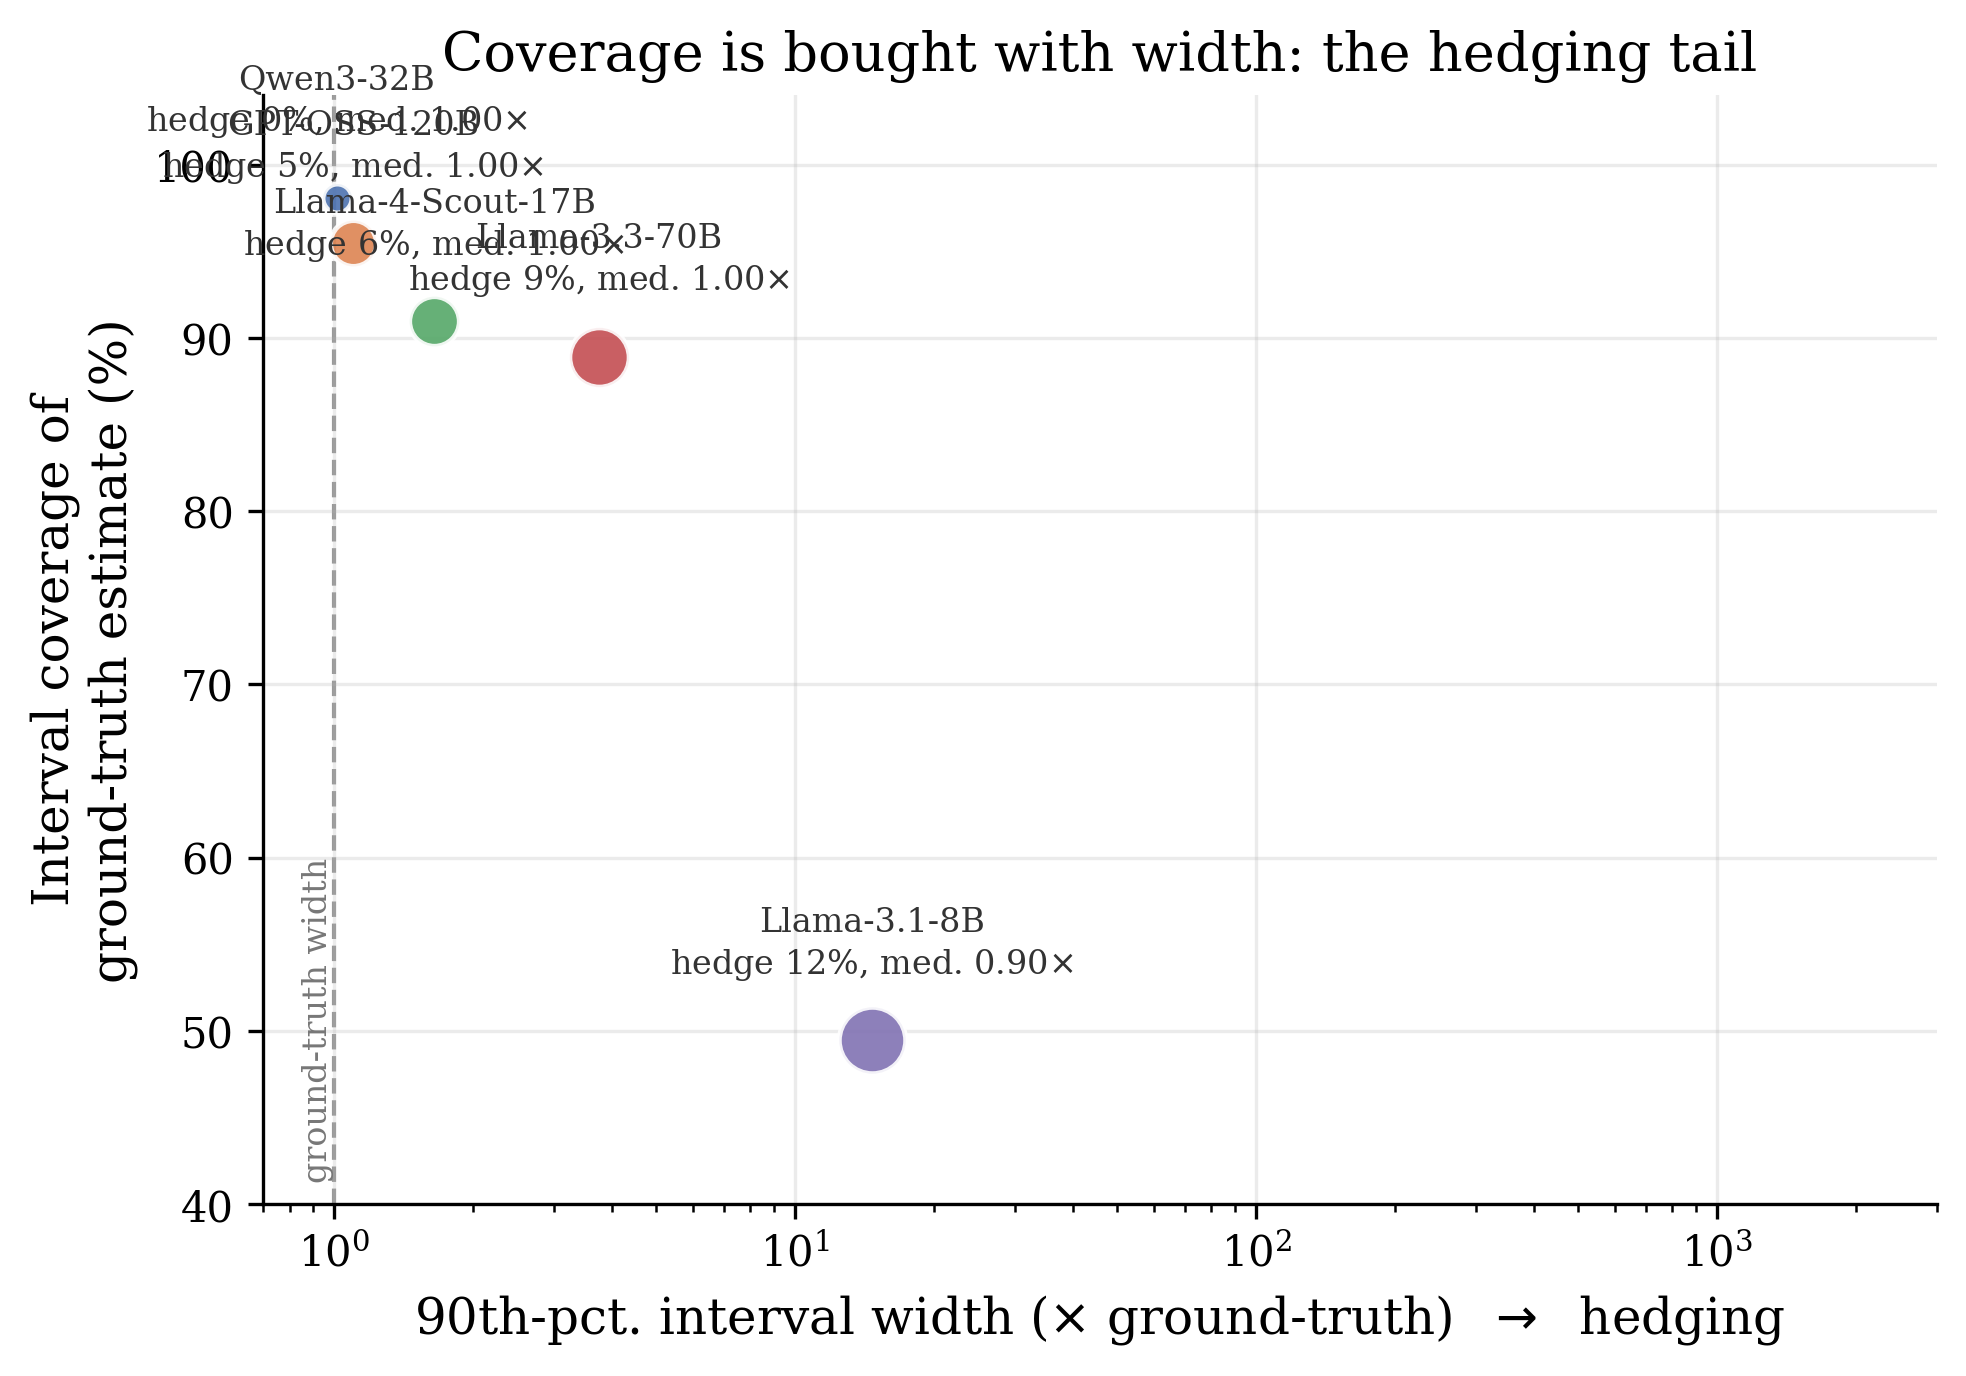
\includegraphics[width=0.72\textwidth]{figures/coverage_sharpness.png}
\caption{Interval coverage against the hedging tail. The horizontal axis is the 90th-percentile interval width in multiples of the ground-truth width (log scale); the dashed line marks the ground-truth width itself. Marker area encodes the hedge rate. The median axis is not shown because it is uninformative---every model sits at $\approx 1.0$---so the separation visible here exists entirely in the tail. Upper left is genuine skill; movement to the right is coverage purchased with uninformative intervals. Note the axis range: after the unit correction of Section~\ref{sec:real_llm_units} the panel spans $1.0\times$ to $14.7\times$ rather than the $6\times$ to $998\times$ the uncorrected intervals showed, and only Llama-3.1-8B sits meaningfully to the right.}
\label{fig:coverage_sharpness}
\end{figure}

\subsection{Accuracy and Calibration Are Separable}
\label{sec:real_llm_calibration}

The panel's principal negative result is that Accuracy@CI and Expected Calibration Error are \emph{separable}. Ranking the five models by each gives a Spearman rank correlation of $\rho = -0.10$ (exact permutation $p = 0.95$), and the same $-0.10$ for debiased ECE, which carries no finite-$n$ floor. The ordering is not merely noisy, it is close to orthogonal: Llama-3.3-70B sits ten accuracy points below the leader with the panel's best ECE ($0.051$ against GPT-OSS-120B's $0.067$), and Qwen3-32B is second on accuracy and fourth on calibration. The only monotone structure in the (accuracy, ECE) plane is at the bottom, where Llama-3.1-8B is worst at both by a wide margin.

This is the reverse of what the same five runs said before the unit correction of Section~\ref{sec:real_llm_units}, where the leaderboard gave $\rho = -0.90$ and we would have reported miscalibration as dominated by capability. The mechanism is direct. The unit artifact marked confidently-correct answers as confidently-wrong, and it did so unevenly across the panel --- worth $+10.6$ points to Qwen3-32B and $+1.4$ to Llama-3.1-8B. Removing an uneven block of confident errors moves accuracy and ECE together for each row, which is precisely how a spurious coupling is manufactured. We report the corrected value and note that the uncorrected one would have been the more quotable finding.

\paragraph{What still tracks accuracy, and why that is not calibration.} Two metrics remain perfectly monotone in Accuracy@CI: the overconfidence rate ($\rho = -1.00$, $p = 0.017$) and the Brier score ($\rho = -1.00$). Neither is evidence of coupling, because neither is independent of the error rate. The overconfidence rate factors exactly as $\Pr(\text{wrong}) \times \Pr(\text{confident} \mid \text{wrong})$, and on this panel the second factor is $82$--$100\%$ with no trend in capability, so the rate is the error rate times a near-constant. The Brier score is a mean squared error against the outcome, and with stated confidence nearly constant across problems (Section~\ref{sec:real_llm_metrics}) it is dominated by the same quantity. ECE and its debiased variant are the metrics in the harness that isolate calibration \emph{shape} from error \emph{volume}, and those are the two that do not follow accuracy.

The distinction matters beyond this panel, because a leaderboard reporting only accuracy-like calibration proxies will show a tight capability/calibration relationship whether or not one exists. It is also the sharpest available answer to the question of why \muru{} should exist alongside accuracy-only mathematical benchmarks: on the panel we measured, knowing a model's accuracy tells you nearly nothing about its calibration in level ($\rho = -0.10$), and nothing at all about whether its confidence discriminates its own correct answers from its wrong ones ($\rho = -0.30$ for AUROC, $p = 0.68$). Two qualifications bound the claim. The panel is five models, so a null correlation at $n = 5$ is weak evidence of absence rather than strong evidence of independence; the honest statement is that the coupling we would have reported is not supported, not that independence is established. And one of the five rows is short of full coverage (245 of 301 problems, difficulty-representative but wider-intervalled), on a permanently withdrawn endpoint. Expanding the panel is the first item of follow-on work, and Section~\ref{sec:limitations} states what it would take to make either reading testable.

\subsection{Difficulty Scaling: Where Real Models Drop}
\label{sec:real_llm_difficulty}

Table~\ref{tab:real_llm_difficulty} resolves the per-difficulty profile of each model. The gradient is real but shallow at the top of the panel: GPT-OSS-120B holds 93--100\% across all five bands, and its lowest cell is D3 (93.3\%) rather than D5 (92.9\%, $n = 28$), so its errors are not where difficulty says they should be --- they are where the categories are (Section~\ref{sec:real_llm_category}). Llama-3.3-70B shows the clearest monotone decline in the panel: 96.2\% on D1 to 64.3\% on D5 ($n = 28$), a 32-point graded drop with no step change, consistent with compounding uncertainty propagation rather than a single hard construction. Llama-4-Scout-17B declines similarly but with its largest step at D2$\to$D3 (97.3\% to 82.0\%) rather than at the adversarial band. Qwen3-32B is the flattest of the four stronger models across D1--D4 (86--96\%) and scores 100\% on D5, but its D5 cell is the smallest in the table ($n = 18$, from the partial-coverage row) and should not be read as evidence that adversarial structure is easy for it. Llama-3.1-8B is flat for a different reason: 35.7--51.4\% across every band, with no ordering that tracks difficulty at all, which is the signature of a model answering from surface statistics rather than from problem-specific reasoning depth.

Two caveats attach to reading these rows as a difficulty curve. The D5 cells carry 18--28 problems each, so single-band comparisons between adjacent models are not resolvable. And the design intent for D5 --- isolating adversarial overconfidence from raw computation depth --- is only partly borne out: three of the five models have their weakest band at D5, but the category decomposition below explains more of the variance than the difficulty label does.

\subsection{Per-Category Profile}
\label{sec:real_llm_category}

Table~\ref{tab:real_llm_category} decomposes Accuracy@CI by category, and it explains more of the panel's error than the difficulty ladder does. Two categories carry nearly all of it. Decision-Under-Uncertainty is the hardest category for three of the five models (GPT-OSS-120B 88.7\%, Llama-4-Scout-17B 77.4\%, Llama-3.3-70B 77.4\%, Qwen3-32B 76.3\%, Llama-3.1-8B 34.6\%), and Adversarial Ambiguity is the hardest for the other two (Llama-3.3-70B 70.2\%, Llama-4-Scout-17B 76.1\%). Against them, the three computational categories --- Bayesian Updating, Conditional Chains, Distribution Estimation --- sit at 90--100\% for every model above the 8B reference. The spread within a single row reaches 30 points (Llama-3.3-70B: 70.2\% on Adversarial Ambiguity against 97.7\% on Conditional Chains), which is the pattern a single aggregate score cannot show.

This is a weaker claim than the one the uncorrected scoring supported, and the difference is instructive. Before the unit correction the same table showed Llama-3.3-70B at 22.6\% and Qwen3-32B at 28.9\% on Decision-Under-Uncertainty --- a category-shaped cliff, and a far more striking result. Most of that gap was the dollar-denominated stems of that category being answered in dollars (Section~\ref{sec:real_llm_units}). What remains is a real but ordinary weakness: the two categories that require composing two independent uncertainties, or acknowledging that more than one formalisation is defensible, are the two where models lose ground. Decision-Under-Uncertainty problems require value-of-information and expected-utility computations over both states and outcomes, and the residual errors we inspected collapse the joint to a point estimate --- the F2 failure catalogued in Section~\ref{sec:failures}. Distribution Estimation remains the easiest category for every model in the panel ($\geq 92\%$ throughout, 100\% for the two strongest): it exercises one closed-form interval computation per problem and requires no composition.

\subsection{Framework-Match on Partial-Coverage Rows}
\label{sec:real_llm_anomalies}

The framework-match rate is computed only over predictions that actually carry a framework field. This matters for rows whose coverage was accumulated across daily budget windows: a small number of early answers were recovered from progress logs (the salvage path) that preserve the parsed point estimate and stated confidence but not the raw response text, so the reasoning framework cannot be re-extracted for those specific problems. We treat such entries as \emph{missing data} for the framework metric---excluded from the denominator---rather than scoring them as incorrect, which would spuriously depress the rate. The effective framework sample size is annotated in Table~\ref{tab:real_llm_main} where it falls below the answered-problem coverage (e.g.\ GPT-OSS-120B reports framework-match over the $n = 222$ freshly-queried answers within its complete $n = 301$ accumulated run, and Qwen3-32B over $n = 212$ within its $n = 245$ run). The point-estimate-derived metrics (Accuracy@CI, ECE, overconfidence) use the full answered subset and are unaffected. All framework fields for the fully-completed portion of every run are preserved in the on-disk archive at write time, so this correction shrinks toward zero as coverage completes.

\subsection{Reproducibility}
\label{sec:real_llm_repro}

Every row of Table~\ref{tab:real_llm_main} can be regenerated from a single JSON archive shipped with the repository:
\begin{enumerate}[leftmargin=*,itemsep=1pt]
\item Set the appropriate API key (\texttt{GROQ\_API\_KEY} for Groq-hosted models or \texttt{OPENROUTER\_API\_KEY} for OpenRouter-hosted models).
\item Run \texttt{python evaluation/run\_eval.py --model <name> --save} to produce a fresh JSON archive in \texttt{evaluation/baselines/}. Problems are evaluated in a seeded-shuffled order; adding \texttt{--resume} skips problems already answered in prior archives for the model and merges the new answers in, so a run split across several free-tier daily-token windows accumulates toward full coverage rather than re-querying (the four accumulated rows in Table~\ref{tab:real_llm_main}---Llama-3.3-70B, GPT-OSS-120B, Qwen3-32B, and Llama-3.1-8B---were built this way).
\item Run \texttt{python evaluation/aggregate\_real\_llm.py} to recompute the bootstrap intervals and refresh every \texttt{paper/tables/real\_llm\_*.tex} include. This step alone, with no API key and no network access, rebuilds every number in this section from the committed archives.
\end{enumerate}
The aggregator emits one LaTeX include per table, so adding a new row to the leaderboard is a one-step operation. One caveat applies to step 2 beyond endpoint availability: the archived panel was collected under prompt version~1, which did not state the unit convention (Section~\ref{sec:real_llm_units}). \texttt{run\_eval.py} now ships version~2, which does, and stamps \texttt{prompt\_version} into every archive it writes. A fresh run is therefore a version~2 run and is not bit-comparable to the archived rows; on a version~2 archive the unit accounting is expected to be the identity, and Section~\ref{sec:real_llm_promptv2} reports the replication that confirms it (zero corroborated unit mismatches under version~2 on both models that follow the instruction). The full set of raw responses, parsed predictions, and computed metrics for the panel reported here is committed to the repository, so the leaderboard is replicable bit-exactly without re-running any API calls.

\paragraph{Endpoint availability.} Step 2 is the one part of this recipe that a provider can invalidate, and during the preparation of this paper it did, four times. As of 2026-08-03 the Groq roster no longer served \texttt{qwen/qwen3-32b} or \texttt{meta-llama/llama-4-scout-17b-16e-instruct}; by 2026-08-17 \texttt{llama-3.3-70b-versatile} and \texttt{llama-3.1-8b-instant} had gone the same way. Requests for any of the four now return \texttt{model\_not\_found}. Of the five endpoints this panel was measured on, one --- \texttt{openai/gpt-oss-120b} --- is still served, so re-running step 2 today reproduces one row rather than five. Two further consequences follow. The Qwen3-32B row is frozen at 245/301: its remaining 56 problems cannot be queried on this provider, which is why that row is reported at partial coverage rather than carried to completion like the rest of the panel. And the prompt-version replication of Section~\ref{sec:real_llm_promptv2} lost two of its three arms while they were running, which is why two rows of Table~\ref{tab:prompt_versions} are paired on fewer than 100 problems.

We report the dates because the interval is the finding: four of five endpoints withdrawn in fourteen weeks is not an unlucky draw, it is the expected service life of a free-tier hosted model, and any benchmark whose numbers are only reproducible by re-querying such endpoints has a shelf life measured in months. This is the reason we commit every raw API response rather than only the computed metrics: steps 1 and 2 are optional, step 3 alone reconstructs every number in this section from the archives, and that path is unaffected by provider roster changes. It is also the reason the archives are the artefact we ask reviewers to check, rather than a re-run. Researchers wanting to extend the panel should expect to substitute currently-served identifiers; the harness resolves display names to provider identifiers through a single \texttt{MODEL\_MAP} table, so a substitution is a one-line change --- but a substituted endpoint is a new row, not a reproduction of an old one.


\section{Failure-Mode Analysis}
\label{sec:analysis}

\subsection{Failure-Mode Taxonomy}
\label{sec:failures}

The benchmark is built around four failure modes drawn from the uncertainty-reasoning literature. Each problem's \texttt{common\_failure\_modes} field records which of the four (and which template-specific variants) the problem is designed to elicit. We summarise the taxonomy here together with the patterns the language-model leaderboard in Section~\ref{sec:real_llm} actually exhibits.

\paragraph{F1: Anchoring on surface statistics.} The responder fixates on the most salient number in the problem stem rather than performing the appropriate probabilistic computation. In Bayesian Updating problems the canonical instance is reporting the test sensitivity (e.g.\ 95\%) instead of the posterior probability, which is the standard base-rate-neglect fallacy. The Llama-3.1-8B row in Table~\ref{tab:real_llm_category} (Bayesian Updating accuracy of 23.0\%, the lowest in the panel) is consistent with this failure mode dominating its responses on Bayesian problems, even as it scores 92.2\% on Distribution Estimation problems where no base rate is involved.

\paragraph{F2: Ignoring compound uncertainty.} D4 and D5 problems propagate uncertainty through several layers (uncertain prior, uncertain likelihood, uncertain sample size). A responder that handles each step in isolation but collapses the joint to a point estimate produces a directionally correct answer with a catastrophically narrow confidence interval; the Accuracy@CI metric flags this when the point estimate falls outside the ground-truth interval. The Decision-Under-Uncertainty column in Section~\ref{sec:real_llm_category} (76.3--88.7\% for the four stronger models, against 97--100\% on Conditional Chains) is the clearest empirical trace of this failure on our panel: the same models that are at or near the ceiling on single-uncertainty categories lose ground on the value-of-information template, which requires composing uncertainty over states with uncertainty over outcomes. The effect is real but ordinary in size; an earlier version of this analysis put it at 22.6--28.9\% for two of the rows, and most of that gap was the unit artifact of Section~\ref{sec:real_llm_units} rather than a reasoning failure.

\paragraph{F3: Single-formalisation commitment.} Adversarial Ambiguity problems admit several defensible formalisations (Simpson's-Paradox-style aggregate-versus-subgroup conflicts, reference-class problems). A responder that commits to one formalisation with high stated confidence is penalised both by Accuracy@CI (whose ground-truth interval spans the defensible range) and by the overconfidence rate. Adversarial Ambiguity is the weakest category for Llama-3.3-70B (70.2\%) and Llama-4-Scout-17B (76.1\%), and the second-weakest for Qwen3-32B (84.4\%), which is consistent with this failure mode being the binding constraint at the top of the panel. It is also the category where the four-field output schema works against the responder: a model that correctly identifies two defensible formalisations still has to report one point estimate, so the schema cannot distinguish acknowledged ambiguity from unrecognised ambiguity. Section~\ref{sec:conclusion} lists this as an open question rather than a settled failure attribution.

\paragraph{F4: Framework confusion.} Applying frequentist machinery where Bayesian machinery is appropriate, or vice versa. The framework-match metric is designed to surface this failure independently of whether the numerical answer falls in range. All rows of Table~\ref{tab:real_llm_main} place framework-match rates between 77\% and 93\% (computed over each row's framework-carrying answers; see Section~\ref{sec:real_llm_anomalies}), indicating that framework selection is not the bottleneck on the panel we evaluated: models identify the correct machinery far more often than they execute it correctly, so the accuracy gaps are driven by computation rather than by framework confusion.

\subsection{Calibration-Metric Behaviour}
\label{sec:calibration}

\begin{wraptable}{r}{0.45\textwidth}
\vspace{-12pt}
\centering
\caption{Calibration metrics from the simulator profile (Section~\ref{sec:results}).}
\label{tab:calibration}
\begin{tabular}{lcc}
\toprule
\textbf{Tier (simulated)} & \textbf{ECE}$\downarrow$ & \textbf{OvConf}$\downarrow$ \\
\midrule
Random & 0.515 & 36.2\% \\
Heuristic & 0.470 & 44.5\% \\
Competent & 0.239 & 21.6\% \\
Strong & 0.178 & 20.3\% \\
Expert & 0.183 & 9.6\% \\
\bottomrule
\end{tabular}
\vspace{-12pt}
\end{wraptable}

Table~\ref{tab:calibration} reproduces the simulator-tier calibration metrics from Section~\ref{sec:results}, against which the language-model rows in Table~\ref{tab:real_llm_main} should be read. The simulator was configured to admit accuracy/calibration dissociation: the Strong and Expert tiers share an ECE band (around 0.18) despite a 16-point accuracy gap. That configuration turns out to have been the more realistic one. Real models in Table~\ref{tab:real_llm_main} do not lie on a diagonal in the (Accuracy@CI, ECE) plane: the rank correlation across the panel is $\rho = -0.10$, and the two best-calibrated rows are the third- and fourth-most accurate. The simulator therefore validates the harness in the relevant sense---it demonstrates that the metrics \emph{can} move independently, which is what makes a null correlation on real models interpretable rather than a property of the instrument. The overconfidence rate does move monotonically with accuracy (50.2\% on Llama-3.1-8B versus 3.0\% on GPT-OSS-120B, a $16.8\times$ reduction in safety-relevant high-confidence-wrong responses), but Section~\ref{sec:real_llm_calibration} shows why that is close to arithmetic rather than evidence of coupling: the rate is the error rate multiplied by a factor that is flat across the panel. One qualification carries across all of these metrics and is developed in Section~\ref{sec:real_llm_metrics}: they all measure calibration \emph{in level}, and none of them measures whether stated confidence discriminates correct answers from incorrect ones. On that separate axis the whole panel performs at or below chance, so a low ECE on this leaderboard should be read as ``this model's confidence is not systematically inflated'', never as ``this model knows when it is wrong''.

\subsection{Statistical Power of the Test Set}
\label{sec:discriminability}

A benchmark of this size has to be able to detect meaningful capability differences. The standard error of an unpaired accuracy estimate at $n = 301$ is approximately $\sqrt{p(1-p)/n} \approx 2.9$ percentage points at $p = 0.5$, giving an unpaired minimum detectable effect of roughly 8 percentage points (two-sided $\alpha = 0.05$). Head-to-head comparisons are paired (every model sees the same 301 problems), so the relevant test is paired McNemar (Table~\ref{tab:mcnemar}), which recovered all four adjacent simulator-tier gaps at $p < 10^{-3}$ including the smallest configured gap of $\Delta = 11.6$ percentage points. The Llama-3.1-8B-versus-Llama-4-Scout-17B comparison on the language-model panel (Section~\ref{sec:real_llm}) spans 41 percentage points and is comfortably above the minimum detectable effect; the leaderboard ordering does not depend on bootstrap-noise assumptions. Finer discrimination---between two frontier models within a few percentage points of each other---is achievable by pooling the validation split (raising the effective $n$ to 602) or by stratified McNemar within a category or difficulty cell, both of which the harness supports.


\section{Discussion}
\label{sec:discussion}

\paragraph{What the panel results imply.}
The 53-percentage-point spread in Accuracy@CI across the panel establishes that \muru{} discriminates capability. What it does \emph{not} establish, and what we expected it to, is that calibration comes along for the ride. At $\rho = -0.10$ between Accuracy@CI and ECE, a model's accuracy on \muru{} tells you close to nothing about how well its stated confidence is calibrated in level, and the resolution result in Section~\ref{sec:real_llm_metrics} says it tells you nothing at all about whether that confidence discriminates. This is the case for the benchmark, made in the opposite direction from the one we set out to make: if calibration were a corollary of accuracy, a calibration benchmark would be a convenience rather than a necessity, and the accuracy-only benchmarks would already cover it. On the panel we measured it is not a corollary. The operational consequence is unchanged and sharpened by the discrimination result. A downstream system that filters language-model outputs by stated confidence cannot increase accuracy beyond what the underlying model already supplies; it can only reduce coverage. With resolution at or below $0.012$ and AUROC in the $0.44$--$0.58$ band, confidence-thresholded filtering on \muru{} discards nearly as many correct answers as wrong ones. Methods that promise calibration without raising accuracy---temperature scaling, self-consistency thresholds, conformal-prediction wrappers---are therefore not free improvements on this benchmark: all of them are monotone transformations of a confidence signal, and a monotone transformation cannot create discrimination that the signal does not already contain. Their gain has to come from somewhere observable, and on this panel the verbalized-confidence channel is not where it is.

\paragraph{Why the overconfidence metric matters.}
The overconfidence rate is constructed to flag a specific safety-relevant failure: a responder that is high-confidence and wrong. On the panel we measured, the metric collapses $16.8\times$---from 50.2\% on Llama-3.1-8B to 3.0\% on GPT-OSS-120B---over the same accuracy range that drives the leaderboard, and it is the metric most tightly correlated with accuracy. The collapse is not an artefact of the $0.7$ cut: the ratio is at least $16.8\times$ at every threshold from $0.5$ to $0.99$, and the threshold-free mean overconfidence is perfectly monotone in accuracy (Table~\ref{tab:real_llm_overconfidence}). In safety-critical decision-support deployment (medical, financial, legal), this metric directly bounds the frequency of high-confidence-wrong outputs that downstream systems must guard against, and the leaderboard makes the bound numerically specific per model. What it does \emph{not} license is a metacognitive reading, and this is the trap the metric sets. Decomposed as $\Pr(\text{wrong}) \times \Pr(\text{confident} \mid \text{wrong})$, only the first factor moves with capability; every model in the panel, leader included, asserts at least four in five of its errors confidently ($82.4$--$100\%$, no trend in capability). The bound tightens because strong models err less often, not because they hedge when they are about to be wrong. A reader who takes the overconfidence column as a calibration ranking is reading the accuracy column twice.

\paragraph{Why the per-category profile matters.}
The category profile in Table~\ref{tab:real_llm_category} is more actionable than the headline leaderboard: two categories---Decision-Under-Uncertainty (76--89\% for the four stronger models) and Adversarial Ambiguity (70--96\%)---carry nearly all of the remaining error, against 90--100\% on the three computational categories. Within a single row the spread reaches 30 points. That points at specific reasoning operations rather than at general capability: composing two independent uncertainties through an expected-utility computation, and acknowledging that a problem admits more than one defensible formalisation. Single-number leaderboards cannot expose this, and we report it as the practical case for per-category reporting. We also report it more cautiously than we first wrote it. Before the unit correction of Section~\ref{sec:real_llm_units} the same column showed two models below 31\%, and the striking version of this finding was an artifact of dollar-denominated stems. A category-shaped hole is exactly what a units bug looks like in aggregate, which is a general warning for anyone reading a category breakdown: check that the weak category is not simply the one with the unusual answer format.


\section{Limitations}
\label{sec:limitations}

\begin{itemize}[leftmargin=*,itemsep=3pt]
    \item \textbf{Open-weights-only language-model panel.} The leaderboard in Section~\ref{sec:real_llm} covers five free-tier hosted open-weights models. Frontier closed-weights endpoints (GPT-4-class, Claude-class, Gemini-class) are not included; the harness supports them via the unified API client, but their inclusion requires paid API access that is outside the scope of this submission. The accuracy/calibration separation we observe is therefore a statement about five open-weights models and should not be extrapolated to closed-weights endpoints, which are trained with calibration-specific objectives we cannot inspect, without re-measurement.
    \item \textbf{Incomplete coverage on one row.} One of the five language-model rows (Qwen3-32B at 245/301) reflects a run that was accumulating against Groq's free-tier daily-token cap when the endpoint was withdrawn from the provider, and it can no longer be completed on that provider (Section~\ref{sec:real_llm_repro}). Its answered subset is a prefix of the seeded evaluation shuffle, hence an approximately random sample of the split rather than an easy-skewed one (D4+D5 share 24.9\% versus 28.6\%), but its bootstrap intervals describe accuracy on the answered subset rather than on the full split, and they are wider than every other row's. It is also the more accurate half of the single rank inversion discussed in Section~\ref{sec:real_llm_calibration}, so that inversion rests on the row we are least able to tighten. The other four rows attempted all 301 problems; where their parse rate is below 100\%, the shortfall is a model-side output-format failure that is scored, not missing coverage, and Table~\ref{tab:real_llm_accounting} reports the effect of that choice (at most 1.7~pp anywhere in the panel).
    \item \textbf{The panel was collected under an underspecified prompt.} The evaluation prompt used for every row in Section~\ref{sec:real_llm} asked for ``a single number'' without stating the unit convention, and 24.7\% of the recorded errors turned out to be correct answers in an admissible unit (Section~\ref{sec:real_llm_units}). We correct this post hoc, conservatively, requiring the model's own interval to corroborate each rescale; the corrected accuracies are therefore lower bounds, with a further 8.6\% of errors rescaling into range without corroboration. The prompt is fixed for future runs and archives now record a \texttt{PROMPT\_VERSION}. The panel itself cannot be re-collected under the corrected prompt --- four of its five endpoints have since been withdrawn by the provider --- but a 100-problem paired replication was run under version~2 while three were still served, and it supports the correction rather than the raw scoring on both models capable of following the instruction (Section~\ref{sec:real_llm_promptv2}). Three qualifications on that support: it covers a third of the test split, three of five rows, and two of its three arms lost their endpoint mid-run; the weakest model is too unstable under re-prompting to contribute evidence either way; and its own residual unit mismatches show that the prompt fix, like the correction, assumes a model that reads the instruction.
    \item \textbf{Overconfidence is a tail statistic on an accurate panel.} At 97.0\% Accuracy@CI the leading model has nine errors in total, so its overconfidence rate rests on nine events and its confidence-versus-correctness AUROC on a 9-versus-292 split. Small-sample effects therefore bind hardest exactly where the leaderboard is most interesting, and this tightens rather than relaxes as models improve. Interpreting single-model differences at the clean end of the panel requires a larger test split than 301 problems.
    \item \textbf{Verbalized confidence is the only elicitation method measured.} Stated confidence is collected from a single greedy sample under one prompt. The near-zero resolution reported in Section~\ref{sec:real_llm_metrics} is therefore a property of \emph{verbalized} confidence under this protocol, not of the models' internal uncertainty. Token-logprob-derived and multi-sample empirical-frequency confidence are known to disagree with verbalized confidence, and either could carry more signal; measuring that disagreement on \muru{} is the most direct extension of this work and is not attempted here.
    \item \textbf{Single sample, single prompt, single temperature.} Every number in Section~\ref{sec:real_llm} comes from one greedy decode per problem under one prompt template. We therefore report no within-model variance, and we cannot separate prompt sensitivity from model capability: an Accuracy@CI difference between two adjacent rows could in principle be reproduced by rewording the prompt. The leaderboard's 50-pp spread is far too large to be explained this way, but the mid-panel gaps of 2--5 pp are not, and should be read as provisional until repeated-sampling and prompt-variant ablations are run.
    \item \textbf{Interval scoring uses the ground-truth point estimate as the realised value.} The Winkler score in Section~\ref{sec:real_llm_metrics} treats each problem's ground-truth point estimate as the outcome to be covered. For Adversarial Ambiguity problems, where the defensible answer is genuinely an interval rather than a point, this is a conservative simplification that charges a model for width even when the ground truth is itself uncertain, and the normalisation by ground-truth width only partly compensates.
    \item \textbf{Parametric generation.} All 3{,}000 problems are produced by 21 generation templates with closed-form solutions. This guarantees correctness by construction and supports arbitrary expansion, but it also introduces structural patterns that a model trained on the train split could exploit. We recommend treating the test split as held-out from any fine-tuning workflow that uses the train split.
    \item \textbf{English-only.} All problem stems are in English. Cross-lingual evaluation requires translation work outside the dataset's scope.
    \item \textbf{Category scope.} The five categories cover the major types of mathematical uncertainty most relevant to applied probabilistic reasoning, but several important domains are not represented---stochastic processes, information-theoretic uncertainty, measure-theoretic probability among them. Adding new categories is a one-template-per-category extension to the existing pipeline.
    \item \textbf{Ground-truth interval choice on adversarial problems.} For Adversarial Ambiguity problems, the ``correct'' answer depends on which formalisation is adopted. We resolve this by reporting an interval over the defensible formalisations rather than a single point estimate, but the interval boundaries themselves embed a judgement about which formalisations count as defensible.
    \item \textbf{Single curator.} Quality assurance relied on automated schema and semantic-consistency validation, with manual spot-checking by a single curator rather than independent expert review by multiple mathematicians. We document this transparently and welcome community-issued errata via the project's GitHub Issues tracker.
\end{itemize}


\section{Conclusion and Future Work}
\label{sec:conclusion}

We introduced \muru{}, a 3{,}000-problem benchmark for mathematical reasoning under genuine uncertainty, and a six-metric evaluation harness, deterministic parametric generation across 21 templates, stratified train/validation/test splits, a unified API client for six hosting providers, a 26-test pytest suite, continuous-integration configuration, a Datasheet for Datasets, and a Croissant metadata file. The harness validation in Section~\ref{sec:results} establishes, via paired McNemar tests on five simulated capability tiers, that the test split has the statistical power to discriminate tier-scale capability differences as small as 11.6 percentage points at $p < 10^{-3}$. The language-model leaderboard in Section~\ref{sec:real_llm} reports the first measurements on the benchmark for five hosted open-weights models and shows a 53-percentage-point spread in Accuracy@CI alongside a near-zero rank correlation between accuracy and Expected Calibration Error ($\rho = -0.10$).

The headline empirical claim of the paper is a null, and it is the one that justifies the benchmark. On the open-weights panel we measured, accuracy and calibration in level are separable: Spearman $\rho = -0.10$ between Accuracy@CI and ECE, with the second-most-accurate model fourth-best calibrated. The metrics that do move with capability---the overconfidence rate, which collapses $16.8\times$ across the panel, and the Brier score---are functions of the error rate rather than of calibration shape, which is a distinction a benchmark needs several metrics to make and which a leaderboard reporting only one of them cannot make at all. The headline diagnostic claim is that single-number leaderboards mask category-shaped weaknesses: Decision-Under-Uncertainty and Adversarial Ambiguity carry nearly all remaining error (70--89\% for the four stronger models) against 90--100\% on the three computational categories.

Two further results sharpen it. On the orthogonal axis of discrimination---whether a model's stated confidence separates its correct answers from its incorrect ones---the entire panel performs at or below chance (Murphy resolution $\leq 0.012$; AUROC $0.439$--$0.575$, with the panel leader below chance), and this does not improve with capability. Calibration in level and discrimination are therefore both unexplained by accuracy, from opposite directions. And the paper's largest single correction was to its own scoring: because the evaluation prompt asked for ``a single number'' on problems denominated in \$K or in percent, 24.7\% of the panel's recorded errors were correct answers in an admissible unit (Section~\ref{sec:real_llm_units}). Correcting that reordered the leaderboard, turned an apparent accuracy/calibration coupling of $\rho = -0.90$ into the $-0.10$ reported above, converted an apparent Decision-Under-Uncertainty cliff into an ordinary weakness, and dissolved an apparent hedging result in which models appeared to buy coverage with intervals up to $998\times$ too wide. We report the correction as its own accounting rather than folding it in silently, because the same failure is available to any benchmark that grades a free-form numeric answer against a stored constant, and it is invisible in aggregate metrics: it looks exactly like a capability gap in whichever category happens to use abbreviated units.

\paragraph{Open questions admitted by the benchmark.}
(1)~Does the accuracy/calibration separation we observe at $n = 5$ survive a panel large enough to estimate a correlation---and do frontier closed-weights endpoints, trained with more calibration-specific objectives, sit on a different part of the plane?
(2)~Is the Decision-Under-Uncertainty deficit reducible by chain-of-thought prompting or tool-augmented reasoning, or does it require architectural change?
(3)~Can any training intervention raise \emph{discrimination}---Murphy resolution, AUROC of confidence over correctness---rather than only calibration in level? Every model we measured is at or below chance on that axis, and no recalibration method can move it.
(4)~Does the Adversarial Ambiguity weakness reflect a reasoning failure or a reporting one---models that identify multiple defensible formalisations but are forced by the output schema to commit to a single point estimate?

\paragraph{Future work.}
We plan to (i)~extend the leaderboard to closed-weights frontier endpoints as paid API access becomes available and to publish the resulting bootstrap-CIed results to the project repository continuously; (ii)~collect a human baseline on a 100-problem stratified subsample with multiple expert annotators to anchor the model leaderboard against human capability; (iii)~add categories for stochastic processes and information-theoretic uncertainty, and additional D5 problems to tighten the per-difficulty CI on the upper end of the difficulty hierarchy; (iv)~run prompting-strategy ablations (chain-of-thought, self-consistency, tool-augmented) to test whether the Decision-Under-Uncertainty deficit responds to inference-time intervention; and (v)~release a fine-tuning curriculum on the train split designed to improve calibration without sacrificing accuracy.

The full dataset, the 21 generation templates, the evaluation harness, the per-model JSON archives that back the leaderboard, the bootstrap and McNemar scripts, the test suite, and the continuous-integration configuration are released at \url{https://github.com/swetank18/MURU_proj} under CC-BY-4.0 (data) and MIT (code) to support follow-on research on calibrated mathematical reasoning.


\bibliographystyle{plainnat}

\begin{thebibliography}{15}

\bibitem[Cobbe et al.(2021)]{gsm8k}
Karl Cobbe, Vineet Kosaraju, Mohammad Bavarian, Mark Chen, Heather Jun, Lukasz Kaiser, Matthias Plappert, Jerry Tworek, Jacob Hilton, Reiichiro Nakano, Christopher Hesse, and John Schulman.
\newblock Training verifiers to solve math word problems.
\newblock \emph{arXiv preprint arXiv:2110.14168}, 2021.

\bibitem[Hendrycks et al.(2021a)]{math}
Dan Hendrycks, Collin Burns, Saurav Kadavath, Akul Arora, Steven Basart, Eric Tang, Dawn Song, and Jacob Steinhardt.
\newblock Measuring mathematical problem solving with the MATH dataset.
\newblock In \emph{NeurIPS}, 2021.

\bibitem[Hendrycks et al.(2021b)]{mmlu}
Dan Hendrycks, Collin Burns, Steven Basart, Andy Zou, Mantas Mazeika, Dawn Song, and Jacob Steinhardt.
\newblock Measuring massive multitask language understanding.
\newblock In \emph{ICLR}, 2021.

\bibitem[Suzgun et al.(2023)]{bigbench}
Mirac Suzgun, Nathan Scales, Nathanael Sch{\"a}rli, Sebastian Gehrmann, Yi Tay, Hyung Won Chung, Aakanksha Chowdhery, Quoc Le, Ed Chi, Denny Zhou, and Jason Wei.
\newblock Challenging BIG-Bench tasks and whether chain-of-thought can solve them.
\newblock In \emph{ACL Findings}, 2023.

\bibitem[Kadavath et al.(2022)]{kadavath2022}
Saurav Kadavath, Tom Conerly, Amanda Askell, Tom Henighan, Dawn Drain, Ethan Perez, Nicholas Schiefer, Zac Hatfield-Dodds, Nova DasSarma, Eli Tyre, et al.
\newblock Language models (mostly) know what they know.
\newblock \emph{arXiv preprint arXiv:2207.05221}, 2022.

\bibitem[Guo et al.(2017)]{guo2017}
Chuan Guo, Geoff Pleiss, Yu Sun, and Kilian Q.\ Weinberger.
\newblock On calibration of modern neural networks.
\newblock In \emph{ICML}, 2017.

\bibitem[Tian et al.(2023)]{tian2023}
Katherine Tian, Eric Mitchell, Allan Dafoe, Anca Dragan, and Yejin Choi.
\newblock Just ask for calibration: Strategies for eliciting calibrated confidence scores from language models.
\newblock In \emph{EMNLP}, 2023.

\bibitem[Gal and Ghahramani(2016)]{gal2016}
Yarin Gal and Zoubin Ghahramani.
\newblock Dropout as a Bayesian approximation: Representing model uncertainty in deep learning.
\newblock In \emph{ICML}, 2016.

\bibitem[Lakshminarayanan et al.(2017)]{lakshminarayanan2017}
Balaji Lakshminarayanan, Alexander Pritzel, and Charles Blundell.
\newblock Simple and scalable predictive uncertainty estimation using deep ensembles.
\newblock In \emph{NeurIPS}, 2017.

\bibitem[Angelopoulos and Bates(2022)]{angelopoulos2022}
Anastasios~N. Angelopoulos and Stephen Bates.
\newblock Conformal prediction: A gentle introduction.
\newblock \emph{Foundations and Trends in Machine Learning}, 2022.

\bibitem[Lin et al.(2022)]{lin2022}
Stephanie Lin, Jacob Hilton, and Owain Evans.
\newblock TruthfulQA: Measuring how models mimic human falsehoods.
\newblock In \emph{ACL}, 2022.

\bibitem[Liu et al.(2024)]{liu2024}
Houwen Liu, Yizhi Li, Maolin Wang, Jiajun Deng, and Zimu Wang.
\newblock MathBench: Evaluating the theory and application proficiency of LLMs with a hierarchical mathematics benchmark.
\newblock \emph{arXiv preprint arXiv:2405.12209}, 2024.

\bibitem[Chen et al.(2023)]{chen2023}
Wenhu Chen, Ming Yin, Max Ku, Elaine Wan, Xueguang Ma, Jianyu Xu, Tony Xia, Xinyi Wang, and Pan Lu.
\newblock TheoremQA: A theorem-driven question answering dataset.
\newblock In \emph{EMNLP}, 2023.

\bibitem[Xiong et al.(2024)]{xiong2024}
Miao Xiong, Zhiyuan Hu, Xinyang Lu, Yifei Li, Jie Fu, Junxian He, and Bryan Hooi.
\newblock Can LLMs express their uncertainty? An empirical evaluation of confidence elicitation in LLMs.
\newblock In \emph{ICLR}, 2024.

\bibitem[Gebru et al.(2021)]{gebru2021}
Timnit Gebru, Jamie Morgenstern, Briana Vecchione, Jennifer Wortman Vaughan, Hanna Wallach, Hal Daum{\'e}~III, and Kate Crawford.
\newblock Datasheets for datasets.
\newblock \emph{Communications of the ACM}, 64(12):86--92, 2021.

\bibitem[Akhtar et al.(2024)]{croissant2024}
Mubashara Akhtar, Omar Benjelloun, Costanza Conforti, Pieter Gijsbers, Joan Giner-Miguelez, Nitisha Jain, Michael Kuchnik, Quentin Lhoest, Pierre Marcenac, Manil Maskey, Peter Mattson, Luis Or{\'e}-Garc{\'\i}a, Pierre Ruyssen, Rajat Shinde, Elena Simperl, Geoffrey Thomas, Slava Tykhonov, Joaquin Vanschoren, Susheel Varma, Jos van der Velde, Steffen Vogler, Carole-Jean Wu, and Luyao Zhang.
\newblock Croissant: A metadata format for ML-ready datasets.
\newblock In \emph{NeurIPS Datasets and Benchmarks Track}, 2024.

\end{thebibliography}


\appendix

\section{Dataset Statistics}
\label{app:statistics}

\begin{figure}[h]
\centering
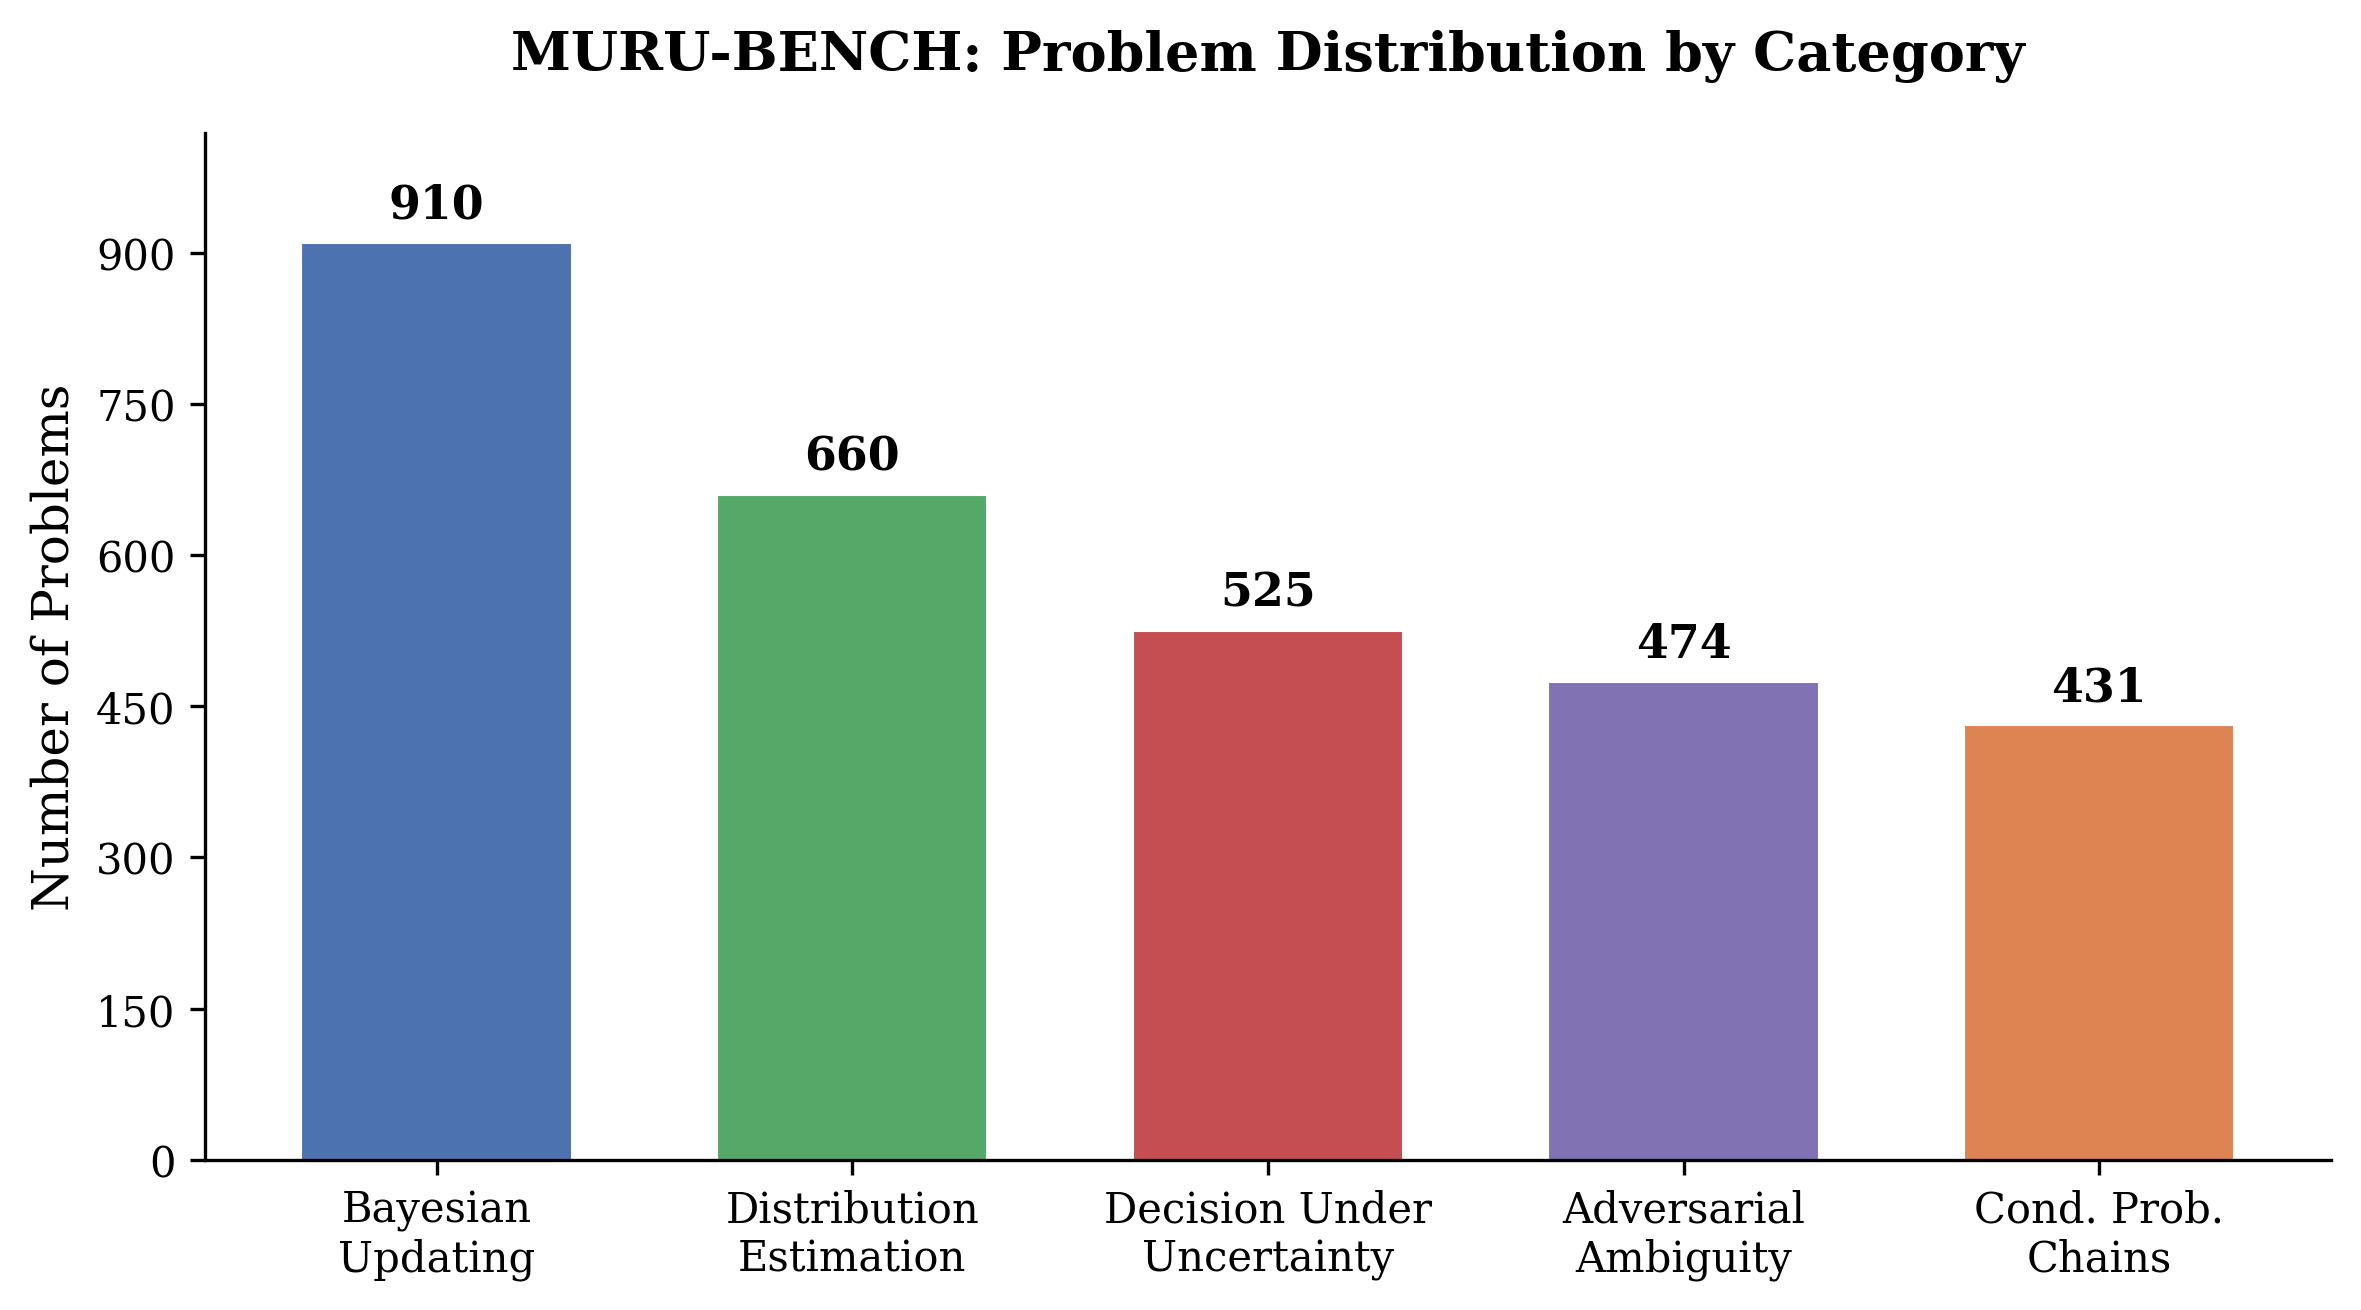
\includegraphics[width=0.7\textwidth]{figures/category_distribution.png}
\caption{Distribution of problems by category in MURU-BENCH. Bayesian Updating is the largest category (910 problems, 30.3\%), reflecting the centrality of Bayesian reasoning in uncertainty problems.}
\label{fig:category_dist}
\end{figure}

\begin{figure}[h]
\centering
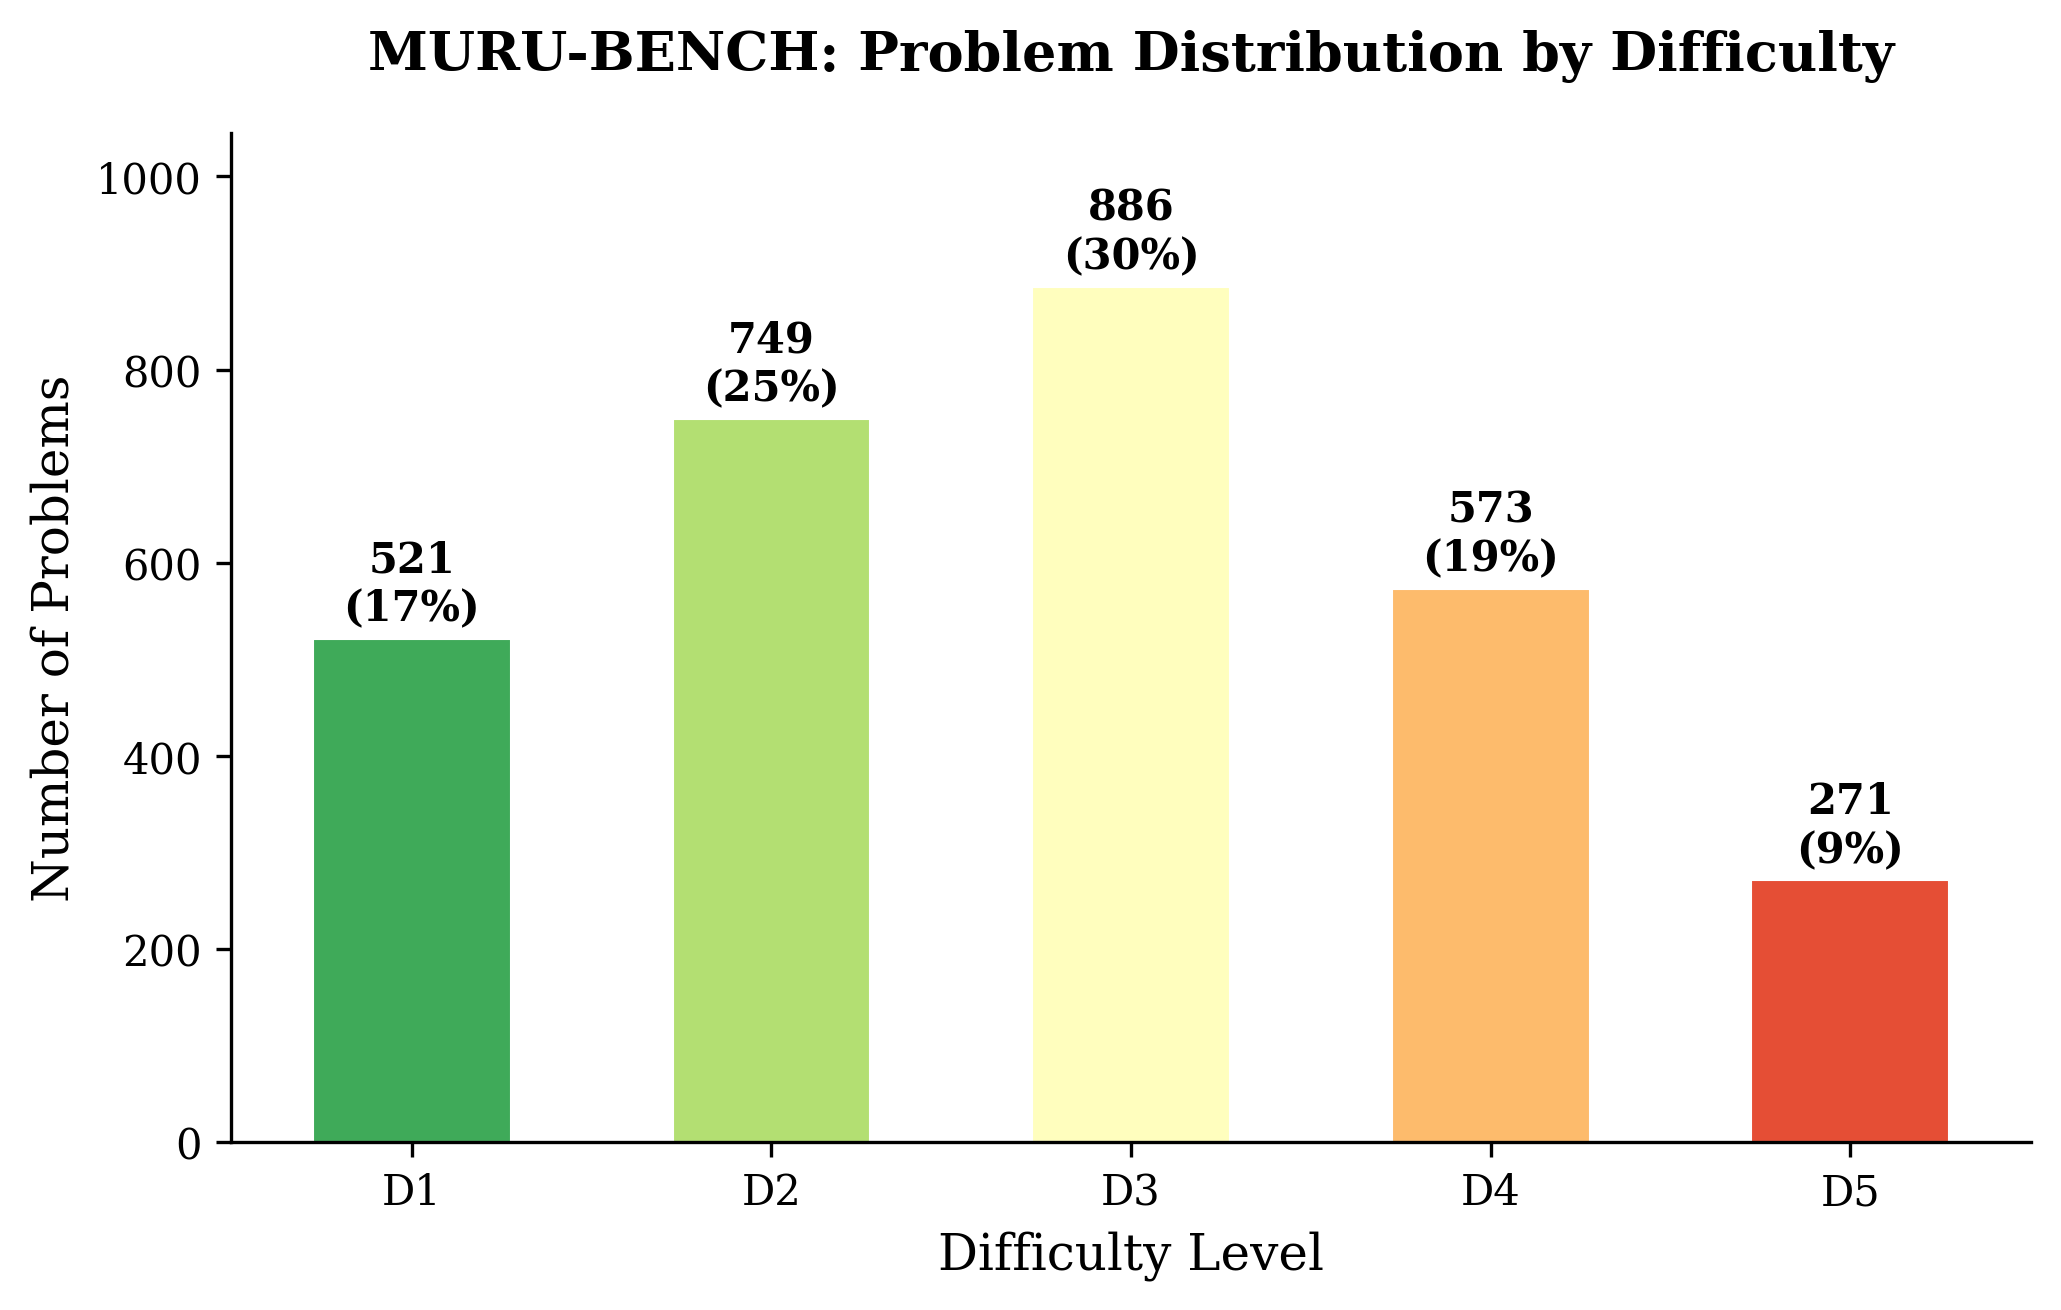
\includegraphics[width=0.6\textwidth]{figures/difficulty_distribution.png}
\caption{Distribution of problems by difficulty level. The distribution is roughly bell-shaped, centred at D3 (886 problems, 29.5\%). D5 problems (271, 9.0\%) are deliberately fewer because they are the most expensive to validate and the most variable in defensible-answer-interval width.}
\label{fig:difficulty_dist}
\end{figure}

\begin{figure}[h]
\centering
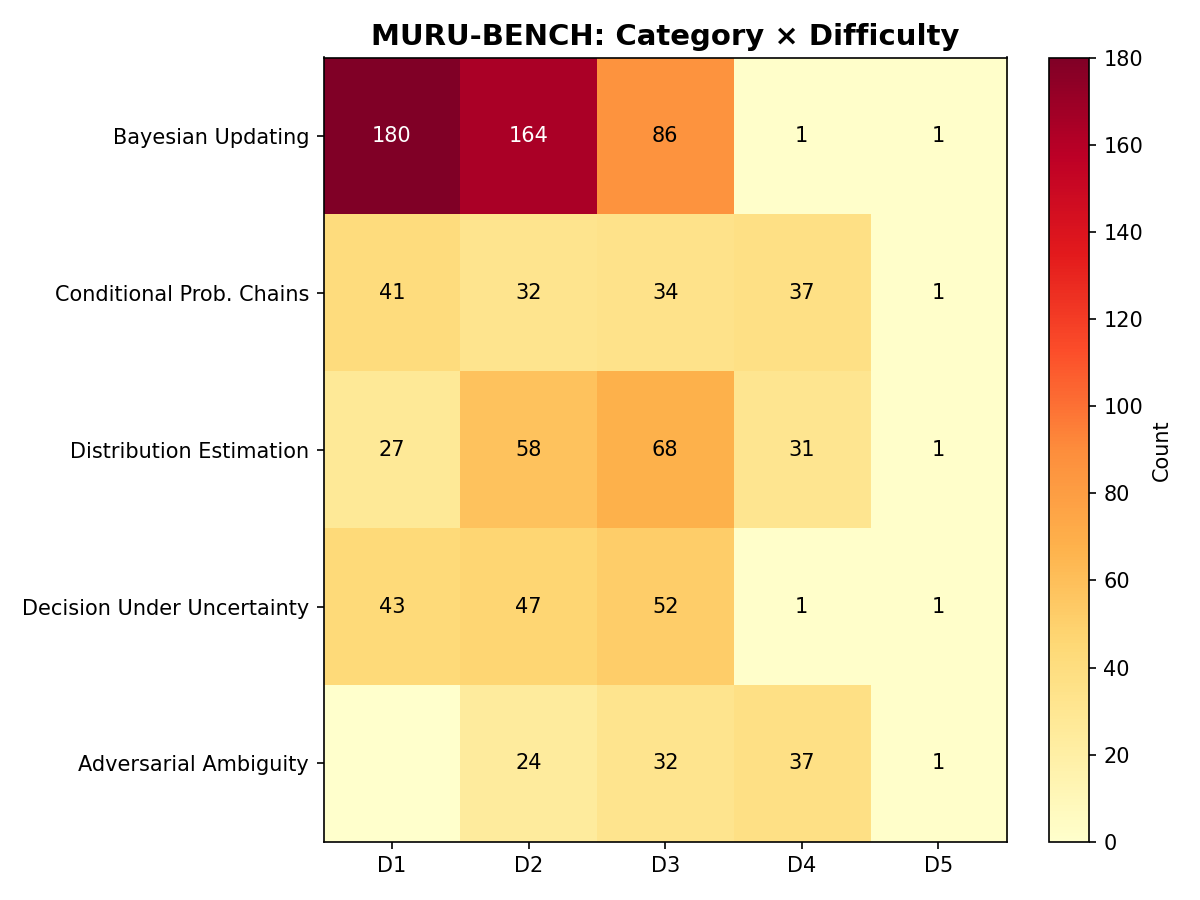
\includegraphics[width=0.7\textwidth]{figures/category_difficulty_heatmap.png}
\caption{Category $\times$ difficulty distribution matrix. Adversarial Ambiguity has no D1 problems by design: recognising structural ambiguity is inherently non-trivial. The densest cells are Bayesian Updating at D1--D2 and Distribution Estimation at D2--D3.}
\label{fig:heatmap}
\end{figure}

\begin{figure}[h]
\centering
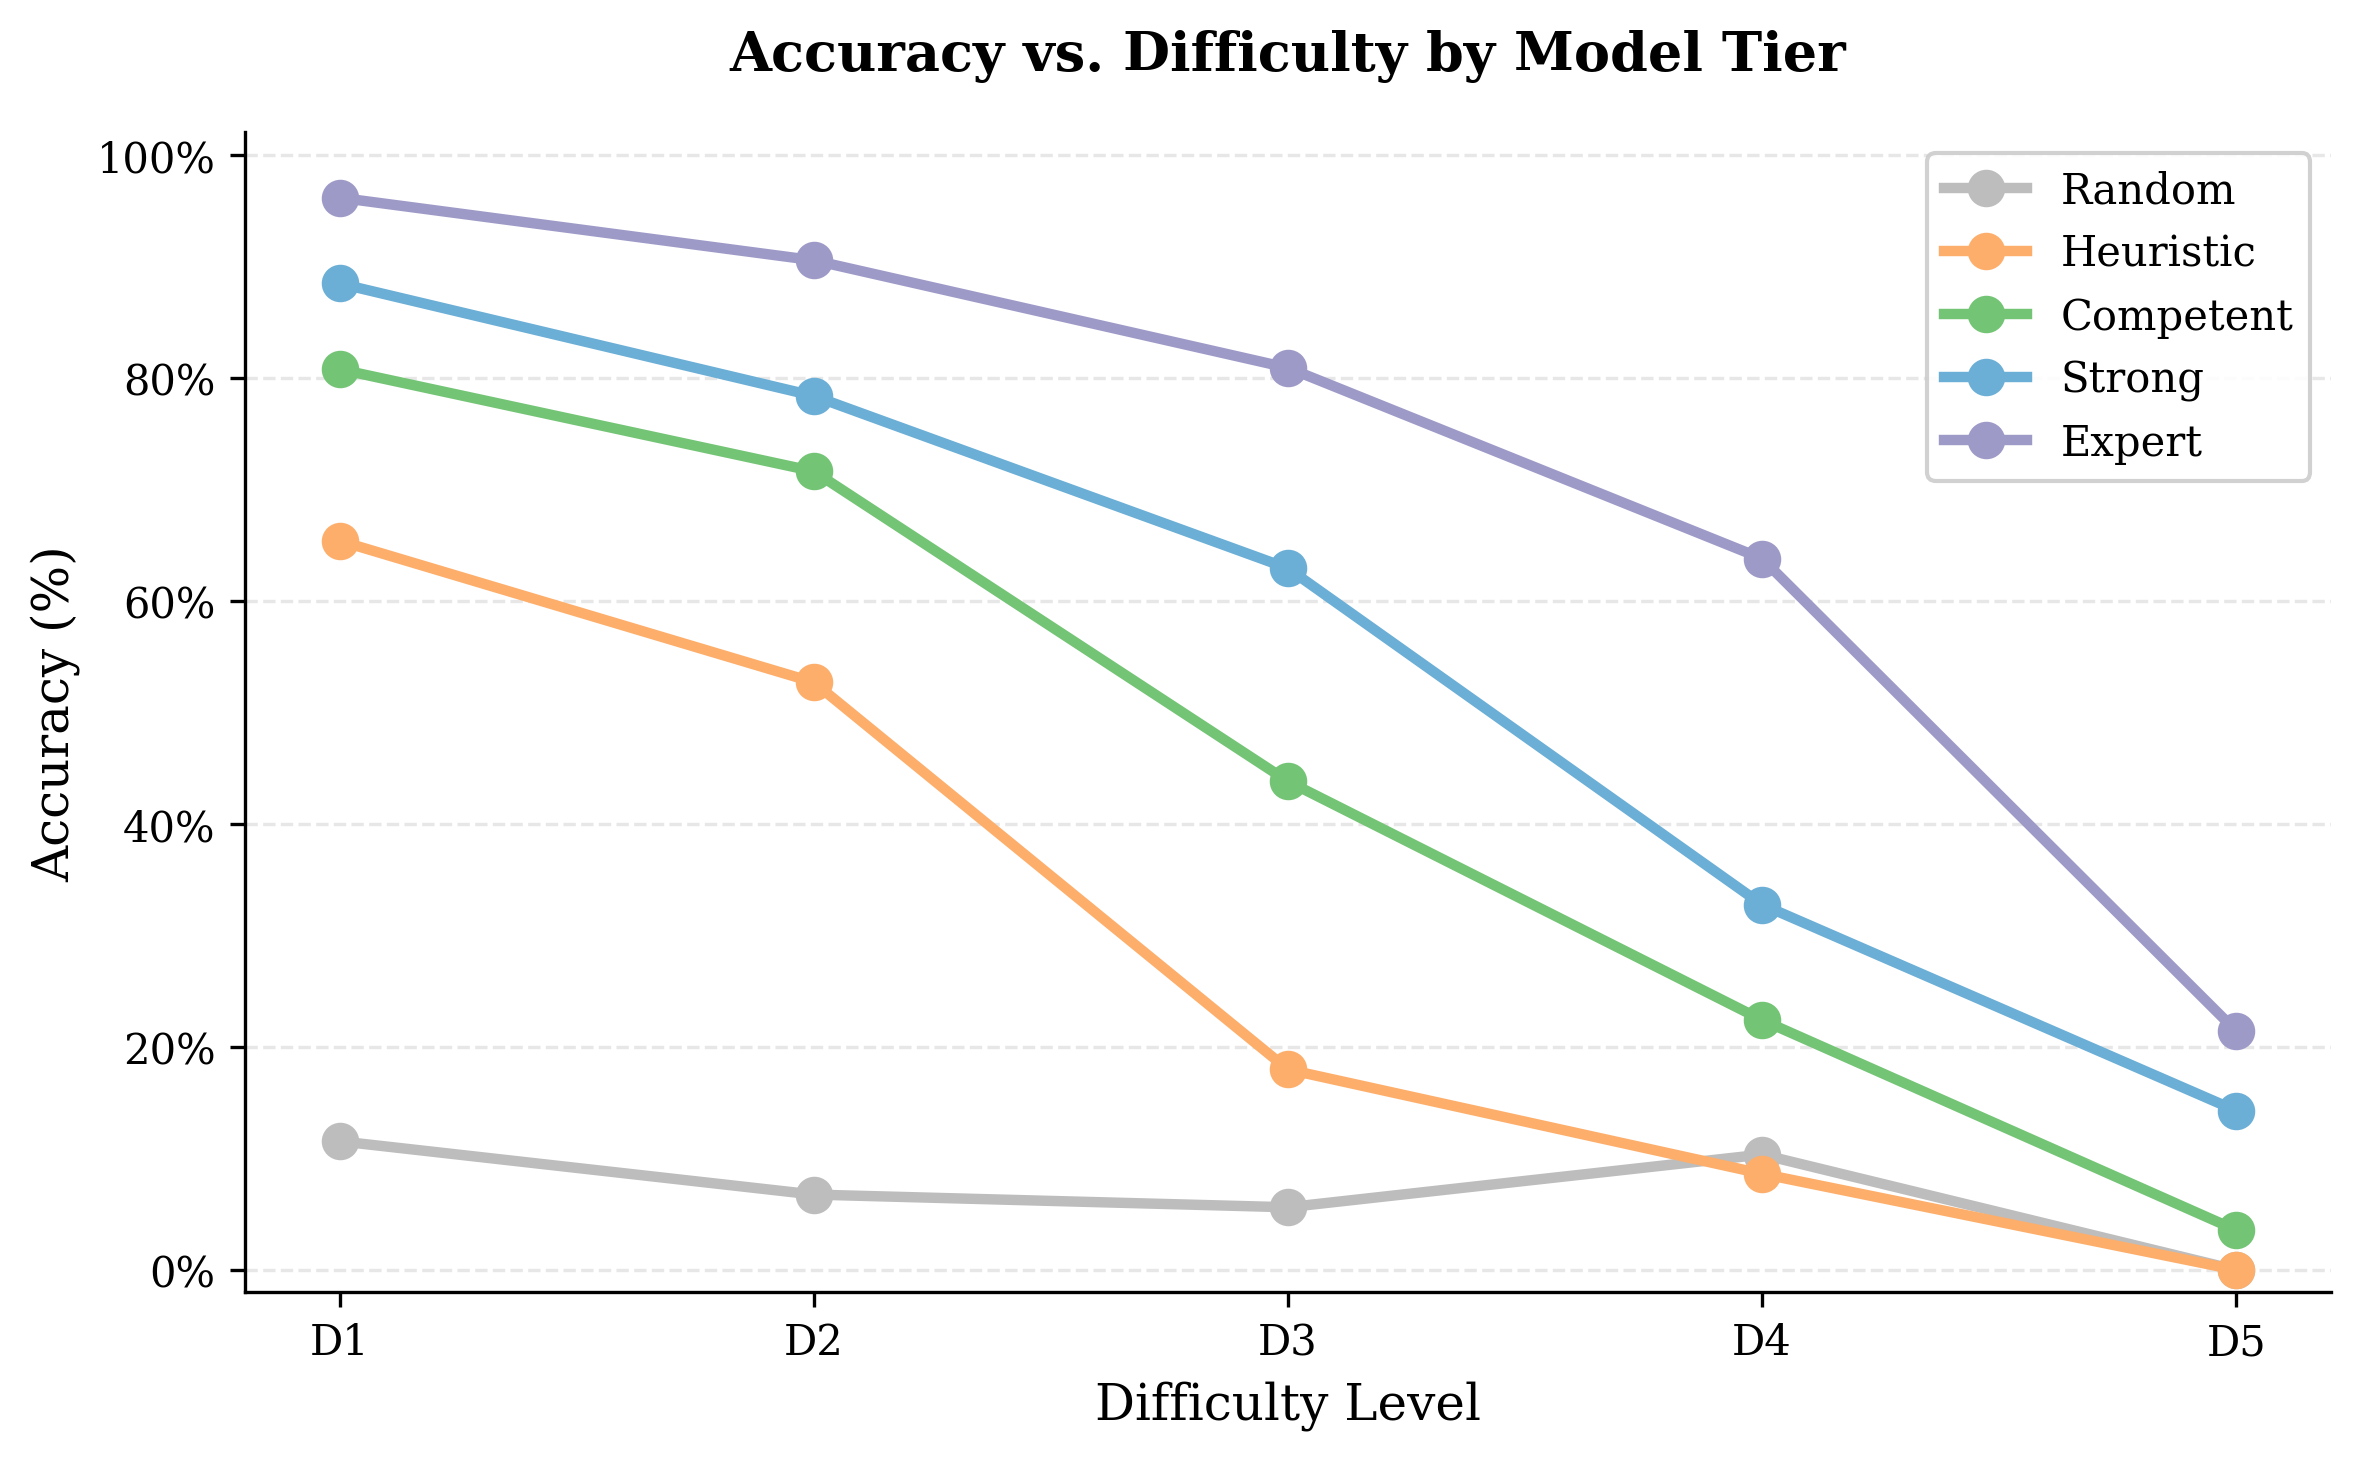
\includegraphics[width=0.75\textwidth]{figures/difficulty_scaling_curve.png}
\caption{Accuracy versus difficulty level by simulator tier. All tiers exhibit monotone accuracy decay. The Expert tier drops from 96\% on D1 to 21\% on D5, a 75-point gap. The D3 inflection point cleanly separates heuristic responders from reasoning-capable ones.}
\label{fig:difficulty_curve}
\end{figure}

\begin{figure}[h]
\centering
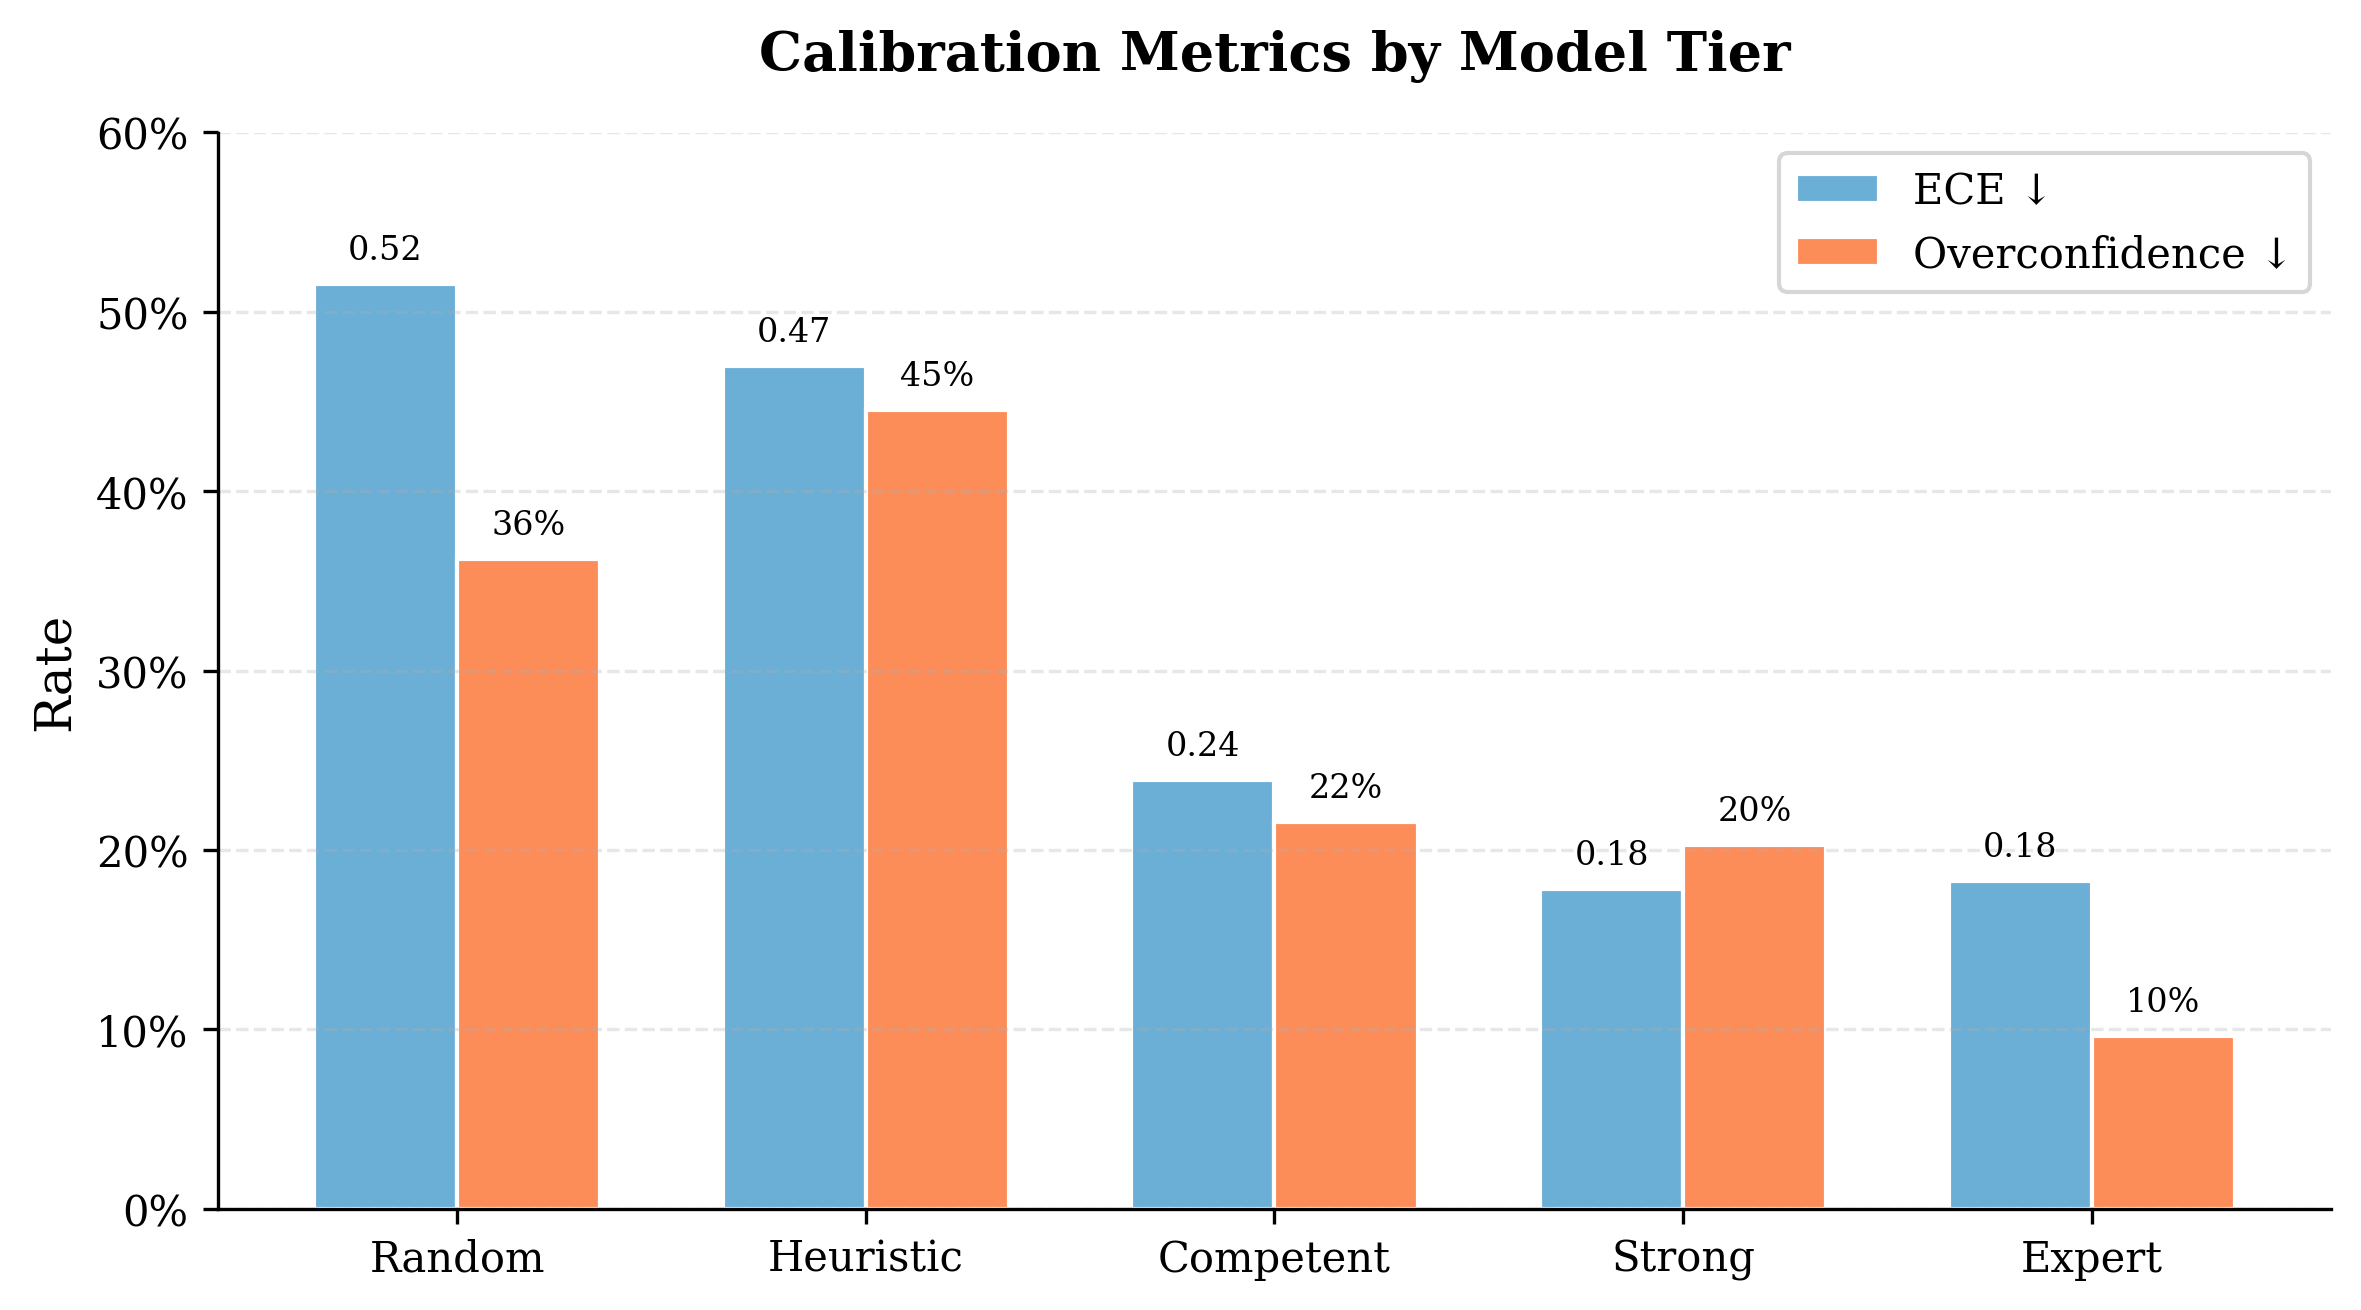
\includegraphics[width=0.75\textwidth]{figures/calibration_comparison.png}
\caption{Calibration metrics by simulator tier. Left bars: ECE ($\downarrow$). Right bars: overconfidence rate ($\downarrow$). The Heuristic tier paradoxically has the highest overconfidence (44.5\%), exceeding even the Random tier; this is what one would expect of a heuristic that confidently outputs answers it has not earned.}
\label{fig:calibration}
\end{figure}


\section{Generation Templates}
\label{app:templates}

Table~\ref{tab:templates} lists all 21 parametric generation templates with their categories, difficulty ranges, and mathematical structures.

\begin{table}[h]
\centering
\caption{All 21 \muru{} generation templates. Each template generates problems with randomised numerical parameters and domain contexts while preserving the underlying mathematical structure.}
\label{tab:templates}
\resizebox{\textwidth}{!}{%
\begin{tabular}{rllcl}
\toprule
\textbf{\#} & \textbf{Template Name} & \textbf{Category} & \textbf{Difficulty} & \textbf{Mathematical Structure} \\
\midrule
1 & \texttt{medical\_test} & Bayesian Updating & D1--D3 & Bayes' theorem with uncertain prevalence \\
2 & \texttt{quality\_control} & Bayesian Updating & D1--D3 & Bayes' theorem for defect rate estimation \\
3 & \texttt{search\_detection} & Bayesian Updating & D1--D2 & Negative evidence updating with uncertain coverage \\
4 & \texttt{sequential\_updating} & Bayesian Updating & D3--D5 & Multiple sequential updates, uncertain likelihood ratios \\
5 & \texttt{hierarchical\_bayes} & Bayesian Updating & D4--D5 & Hierarchical shrinkage, uncertain between-group variance \\
\midrule
6 & \texttt{sequential\_pipeline} & Cond.\ Prob.\ Chains & D1--D4 & Multi-stage pipeline, one uncertain stage \\
7 & \texttt{parallel\_redundancy} & Cond.\ Prob.\ Chains & D2--D4 & $P(\geq 1 \text{ succeeds})$ with common-cause failures \\
8 & \texttt{conditional\_cascade} & Cond.\ Prob.\ Chains & D3--D5 & Branching cascade with uncertain transitions \\
\midrule
9 & \texttt{sample\_mean} & Distribution Estimation & D1--D3 & $t$-distribution CI for population mean \\
10 & \texttt{measurement\_bias} & Distribution Estimation & D2--D4 & Systematic bias correction $+$ sampling CI \\
11 & \texttt{proportion\_estimation} & Distribution Estimation & D1--D3 & Wilson CI, optional stratification \\
12 & \texttt{mixture\_distribution} & Distribution Estimation & D3--D5 & 2-component mixture, uncertain weights \\
13 & \texttt{variance\_estimation} & Distribution Estimation & D2--D4 & $\chi^2$ CI, dual-method comparison \\
\midrule
14 & \texttt{decision\_payoff} & Decision Under Unc. & D1--D3 & Two-option EV with uncertain probability \\
15 & \texttt{multi\_option\_decision} & Decision Under Unc. & D2--D4 & Multi-option EV with sensitivity analysis \\
16 & \texttt{sequential\_decision} & Decision Under Unc. & D3--D5 & Value of information under dual uncertainty \\
17 & \texttt{insurance\_pricing} & Decision Under Unc. & D3--D5 & Poisson frequency $\times$ uncertain severity \\
\midrule
18 & \texttt{base\_rate\_trap} & Adversarial Ambiguity & D2--D4 & High sensitivity $\neq$ high PPV due to low prevalence \\
19 & \texttt{simpsons\_paradox} & Adversarial Ambiguity & D3--D5 & Aggregate vs.\ subgroup with uncertain composition \\
20 & \texttt{reference\_class} & Adversarial Ambiguity & D3--D5 & Multiple valid base rates, no single correct answer \\
21 & \texttt{anchoring\_manipulation} & Adversarial Ambiguity & D2--D4 & Misleading anchor vs.\ data-based correction \\
\bottomrule
\end{tabular}}
\end{table}


\section{Sample Problems}
\label{app:samples}

We present three representative problems to illustrate the benchmark's structure and difficulty scaling.

\subsection*{Example 1: Bayesian Updating (D1)}

\noindent\textbf{Problem.}
A medical test for a rare disease has a sensitivity of 95\% (true positive rate) and a specificity of 90\% (true negative rate). The disease affects 1\% of the population. A patient tests positive. What is the probability that the patient actually has the disease? Express your answer as a probability and provide a confidence interval reflecting the uncertainty in the population prevalence, which epidemiologists estimate could range from 0.5\% to 1.5\%.

\noindent\textbf{Ground truth.}
$P(\text{Disease} \mid \text{Positive})$ ranges from 0.046 to 0.126 depending on the true prevalence (0.5\% to 1.5\%). Point estimate at 1\% prevalence: 0.087. CI level: 90\%.

\noindent\textbf{Required framework.} Bayesian inference.

\noindent\textbf{Common failure modes.}
\begin{itemize}[leftmargin=*,itemsep=1pt]
    \item Ignoring the base rate and reporting the test sensitivity (95\%) as the answer.
    \item Reporting only the point estimate 0.087 without acknowledging prevalence uncertainty.
    \item Confusing sensitivity with positive predictive value.
\end{itemize}

\subsection*{Example 2: Adversarial Ambiguity (D3)}

\noindent\textbf{Problem.}
A coin was flipped 10 times, yielding 7 heads and 3 tails. What is the probability the coin is fair? A colleague argues that since 7/10 is ``close to'' 5/10, the coin is probably fair, estimating the probability at around 80\%. Another colleague uses a frequentist hypothesis test and gets $p = 0.17$, concluding ``we cannot reject the null that the coin is fair.'' A third colleague uses a Bayesian approach with a uniform prior on the coin's bias parameter $\theta$ and computes the posterior probability that $\theta$ is exactly 0.5. Who, if anyone, is reasoning correctly?

\noindent\textbf{Ground truth.}
The question is fundamentally ambiguous. $P(\theta = 0.5 \text{ exactly}) = 0$ under a continuous prior. $P(\theta \in [0.45, 0.55]) \approx 0.11$. The Bayes factor is approximately 0.55. The correct answer depends on which formalisation is adopted, giving a defensible range of $[0.07, 0.55]$.

\noindent\textbf{Required framework.} Bayesian inference (multiple frameworks defensible).

\subsection*{Example 3: Decision Under Uncertainty (D5)}

\noindent\textbf{Problem.}
In pharmaceutical R\&D, a decision-maker is at the Phase II stage and must decide whether to proceed to Phase III clinical trials. The investment cost is \$120M. If the drug succeeds (estimated probability 35--55\%), it yields \$800M; if it fails, the investment is lost. Before deciding, the company can purchase a biomarker study for \$15M. This study correctly predicts success/failure with accuracy 65--80\%. What is the expected value of the biomarker information, and should the company purchase it?

\noindent\textbf{Ground truth.}
The value-of-information depends on both the success-probability range and the biomarker-accuracy range. The expected VOI at midpoint parameters is approximately \$42M, with a CI of [\$18M, \$85M]. Since VoI exceeds the study cost (\$15M) even at the lower bound, the study should be purchased.

\noindent\textbf{Required framework.} Decision theory.


\section{VOI Template Bug Fix}
\label{sec:voi_bug}

During validation, 28 of the initial 2{,}000 generated problems---all from the \texttt{sequential\_decision} template---failed the semantic-consistency check: the point estimate fell outside the confidence interval. Root-cause analysis showed that the value-of-information function is non-monotonic in the uncertain parameters. The CI was computed from the extreme-case scenarios ($p_\text{low}, p_\text{high}$), but the mid-range point estimate could fall outside this range because of the non-linear interaction between success probability and information accuracy.

The fix updated the CI computation to include the mid-range value when determining bounds:
\begin{verbatim}
# Before (incorrect):
ci_vals = sorted([voi_low, voi_high])

# After (correct):
ci_vals = sorted([min(voi_low, voi_high, voi_mid),
                  max(voi_low, voi_high, voi_mid)])
\end{verbatim}

Twenty-eight replacement problems were generated and all 3{,}000 then passed validation. We document this fix as a worked example of the kinds of issues parametric problem generation surfaces, and as transparency about the dataset's history.


\section{Evaluation Prompts}
\label{app:prompts}

All models were evaluated with the following system and user prompts. Temperature was set to 0 for reproducibility.

\subsection*{System prompt}

\begin{quote}
\small
You are a mathematical reasoning expert. You will be given a problem involving mathematical uncertainty. You must:
(1) Identify the correct mathematical framework (\texttt{bayesian\_inference}, \texttt{frequentist\_inference}, \texttt{decision\_theory}, \texttt{information\_theory}, or \texttt{monte\_carlo}).
(2) Show your reasoning step-by-step.
(3) Provide your final answer as a single number (point estimate).
(4) Provide a confidence interval [lower, upper] for your answer.
(5) State your confidence in your answer as a probability between 0 and 1.

Format your response EXACTLY as follows at the end:

\texttt{FRAMEWORK: <framework\_name>} \\
\texttt{POINT\_ESTIMATE: <number>} \\
\texttt{CONFIDENCE\_INTERVAL: [<lower>, <upper>]} \\
\texttt{CONFIDENCE: <probability>}
\end{quote}

\subsection*{User prompt}

\begin{quote}
\small
Problem: \{problem stem\}

Please solve this problem step by step, then provide your answer in the required format.
\end{quote}

Responses are parsed by regex extraction over the four structured fields. Problems whose responses fail to parse are recorded as parse failures and excluded from metric computation but included in the parse-failure rate.


\section{Reproducibility}
\label{app:reproducibility}

All code and data required to reproduce the results in this paper are available at \url{https://github.com/swetank18/MURU_proj}. Key commands:

\begin{verbatim}
# Generate problems
python scripts/generate_problems.py --all --n 3000 --seed 2026

# Split data
python scripts/split_data.py --source data/train/ --seed 42

# Run simulated baselines
python evaluation/run_baselines.py --save

# Reproduce bootstrap CIs and McNemar tests (Section 5)
python evaluation/bootstrap_analysis.py

# Run real model evaluation (requires API keys).
# Problems are evaluated in a seeded-shuffled order (default --seed 42),
# so a run cut short by a hosted-API quota still yields a
# difficulty-representative subset rather than the easy-skewed
# sorted-ID prefix.
python evaluation/run_eval.py --model gpt-4o --save

# Generate analysis and figures
python evaluation/analyze_results.py
python scripts/generate_figures.py

# Run the test suite (metrics, parsing, dataset invariants)
make test
\end{verbatim}

A continuous-integration workflow (\texttt{.github/workflows/ci.yml}) runs the test suite and dataset validation against Python 3.10, 3.11, and 3.12 on every push and pull request. Bootstrap and McNemar results in Section~\ref{sec:results} are bit-for-bit reproduced by \texttt{evaluation/bootstrap\_analysis.py} with seed 42 and 10{,}000 resamples.


\section{Datasheet for Datasets}
\label{app:datasheet}

We follow the Datasheet for Datasets template of \citet{gebru2021}.

\subsection*{Motivation}

\textbf{For what purpose was the dataset created?}
\muru{} was created to support the evaluation of mathematical reasoning under genuine probabilistic uncertainty in language models. Existing mathematical-reasoning benchmarks (GSM8K, MATH, MMLU) treat correctness as deterministic and so cannot measure whether a system reasons correctly about quantities that are themselves probabilistic. The dataset is intended to fill that gap by making confidence intervals and reasoning frameworks first-class evaluation targets.

\textbf{Who created the dataset and on behalf of which entity?}
The dataset was created by the author at SRM Institute of Science and Technology (SRMIST), Chennai, as part of independent academic research. No entity has commercial rights to the dataset.

\textbf{Who funded the creation of the dataset?}
No external funding. Compute and storage were self-provided.

\subsection*{Composition}

\textbf{What do the instances represent?}
Each instance is a self-contained mathematical-reasoning problem expressed in natural-language English, accompanied by closed-form ground truth: a point estimate, a confidence interval at a stated level, an ordered list of solution steps, the required reasoning framework, and a list of expected failure modes.

\textbf{How many instances are there in total?}
3{,}000 problems, partitioned into 2{,}398 train, 301 validation, and 301 test instances by stratified sampling on the (category, difficulty) cross-product.

\textbf{Does the dataset contain all possible instances or is it a sample?}
It is a deterministic sample drawn from 21 parametric generation templates (Appendix~\ref{app:templates}). Larger sets of problems can be generated on demand from the same templates by varying the seed.

\textbf{What data does each instance consist of?}
Each instance is a JSON document conforming to the schema in \texttt{problem\_schema.json}. Fields include \texttt{id}, \texttt{stem}, \texttt{category}, \texttt{difficulty}, \texttt{uncertainty\_type}, \texttt{required\_framework}, \texttt{ground\_truth} (with \texttt{answer}, \texttt{point\_estimate}, \texttt{confidence\_interval}, \texttt{ci\_level}), \texttt{solution\_steps}, \texttt{common\_failure\_modes}, and \texttt{metadata}.

\textbf{Is there a label or target associated with each instance?}
Yes. The label is the \texttt{ground\_truth} object, with a numerical target and a structured confidence interval; the \texttt{required\_framework} field is also a label, used by the framework-match metric.

\textbf{Is any information missing from individual instances?}
No. All fields are populated for all 3{,}000 instances.

\textbf{Are relationships between individual instances made explicit?}
No instance-to-instance relationships are encoded. Within a (category, difficulty) cell, instances are i.i.d.\ samples from the corresponding template.

\textbf{Are there recommended data splits?}
Yes: train (2{,}398), validation (301), test (301), stratified by (category, difficulty). The test split is used for the discriminability analysis in Section~\ref{sec:results}; we recommend reserving it for held-out evaluation in downstream work.

\textbf{Are there errors, sources of noise, or redundancies?}
Validation found and corrected 28 sequential-decision-template instances whose ground-truth interval excluded the mid-range point estimate (Appendix~\ref{sec:voi_bug}). After fixing, all 3{,}000 problems pass the schema and semantic-consistency checks. We are not aware of remaining errors.

\textbf{Is the dataset self-contained, or does it link to external resources?}
Self-contained. All problems are JSON; no external assets are referenced.

\textbf{Does the dataset contain data that might be considered confidential?}
No.

\textbf{Does the dataset contain content that, if viewed directly, might be offensive, insulting, threatening, or otherwise cause anxiety?}
No. Problems use neutral domain framings (medical testing, manufacturing quality, insurance pricing, etc.) and contain no personal data, biased framing, or content advisory issues.

\subsection*{Collection process}

\textbf{How was the data acquired?}
The dataset was synthesised programmatically by 21 generation templates implemented in \texttt{scripts/generate\_problems.py}. Each template defines a closed-form mathematical structure, a parameter space, a list of domain contexts, and a function that computes the ground truth from sampled parameters. No web scraping or human-authored prompts.

\textbf{What mechanisms or procedures were used to collect the data?}
A deterministic Python pipeline using \texttt{numpy.random.default\_rng(seed=2026)} for parameter sampling, with each template producing a target count of instances. Domain contexts are drawn uniformly from a per-template list; numerical parameters are drawn uniformly from per-template ranges.

\textbf{Were any ethical review processes conducted?}
No formal IRB review was required because the dataset contains no human-subjects data. The author self-certifies that the dataset complies with the institution's research-conduct policy.

\textbf{Does the dataset relate to people?}
No.

\subsection*{Preprocessing/cleaning/labelling}

\textbf{Was any preprocessing or labelling done?}
Generation produces labels directly; no separate labelling step. A three-stage validation pipeline (schema, semantic consistency, spot-check; see Section~\ref{sec:qa}) gates problem inclusion. Twenty-eight instances were regenerated after the VOI bug fix.

\textbf{Was the ``raw'' data saved in addition to the cleaned data?}
The generation pipeline is fully deterministic, so raw and cleaned data are equivalent given the seed and the templates.

\textbf{Is the software used to preprocess/clean/label the instances available?}
Yes, at \url{https://github.com/swetank18/MURU_proj} under MIT license.

\subsection*{Uses}

\textbf{Has the dataset been used for any tasks already?}
The dataset has been used to validate the \muru{} evaluation harness via the simulated-tier discriminability study in Section~\ref{sec:results} and to produce the language-model leaderboard in Section~\ref{sec:real_llm}, which reports test-split measurements for five hosted open-weights models with paired-bootstrap 95\% intervals on every metric.

\textbf{What (other) tasks could the dataset be used for?}
Beyond benchmark evaluation, the dataset is suitable for: (1)~fine-tuning curricula targeting calibrated reasoning; (2)~ablation studies of chain-of-thought or tool-augmented reasoning; (3)~studies of metacognitive calibration; (4)~teaching probabilistic reasoning at the undergraduate level.

\textbf{Is there anything about the composition or collection process that might affect future uses?}
Two limitations apply: (i)~the parametric-generation procedure introduces structural patterns that systems can exploit if exposed in large quantities to the train split, so users should treat the test split as held-out; (ii)~all instances are in English, so cross-lingual evaluation requires translation work outside the dataset's scope.

\textbf{Are there tasks for which the dataset should not be used?}
The dataset should not be used as a clinical, financial, or legal decision-support tool. It is a research benchmark; the framings (medical testing, insurance pricing, etc.) are illustrative, not domain-validated.

\subsection*{Distribution}

\textbf{Will the dataset be distributed to third parties outside the entity on behalf of which it was created?}
Yes. The dataset is released publicly under CC-BY-4.0 at \url{https://github.com/swetank18/MURU_proj}. The accompanying code is released under MIT.

\textbf{How will the dataset be distributed?}
Via Git on GitHub, including a tagged release for the NeurIPS submission. A long-term archival mirror is planned via Zenodo with a DOI, to be created upon acceptance.

\textbf{When will the dataset be distributed?}
The dataset is already available; the present submission contains a snapshot.

\textbf{Will the dataset be distributed under a copyright or other intellectual property license?}
Data: Creative Commons Attribution 4.0 International (CC-BY-4.0). Code: MIT.

\textbf{Have any third parties imposed IP-based or other restrictions on the data?}
No.

\textbf{Do any export controls or other regulatory restrictions apply?}
No.

\subsection*{Maintenance}

\textbf{Who will be supporting/hosting/maintaining the dataset?}
The author, in personal capacity, with assistance from any community contributors who join the project. GitHub Issues is the support channel of record.

\textbf{How can the owner/curator/manager of the dataset be contacted?}
Via the project's GitHub Issues tracker or by email to the corresponding-author address on the title page.

\textbf{Is there an erratum?}
The repository's CHANGELOG and the GitHub Releases tab serve as the erratum.

\textbf{Will the dataset be updated?}
Minor updates (bug fixes, additional metadata) will be tagged and announced via GitHub Releases. Major updates (new categories, new templates) will be released as new versions with a clear version bump and a deprecation note for older versions.

\textbf{If the dataset relates to people, are there applicable limits on the retention of the data associated with the instances?}
Not applicable.

\textbf{Will older versions of the dataset continue to be supported/hosted/maintained?}
Yes. All tagged releases remain available indefinitely on GitHub.

\textbf{If others want to extend/augment/build on the dataset, is there a mechanism for them to do so?}
Yes. Pull requests are welcome on the project repository; \texttt{CONTRIBUTING.md} documents the contribution flow.


\section{Author Statement, License, and Intended Uses}
\label{app:author_statement}

\subsection*{Author statement of responsibility}

The author bears all responsibility in case of violation of rights. The author confirms the following:
(a)~no third-party intellectual property, personal data, or restricted material was used to construct the dataset;
(b)~the dataset is released under a permissive license (CC-BY-4.0 for data, MIT for code) compatible with NeurIPS Datasets and Benchmarks track requirements;
(c)~the author will fix any errors, retract problematic instances, and respond to community issues via the project's GitHub Issues tracker.

\subsection*{License}

\textbf{Data:} Creative Commons Attribution 4.0 International (CC-BY-4.0). Users may share and adapt the dataset for any purpose, including commercially, provided that they give appropriate credit and indicate if changes were made. Citation: see Section~\ref{app:citation}.

\textbf{Code:} MIT License. The full license text is included in the repository at \texttt{LICENSE}.

\subsection*{Intended uses}

\muru{} is intended for:
\begin{itemize}[leftmargin=*,itemsep=2pt]
    \item evaluating language models on calibrated mathematical reasoning;
    \item studying the relationship between reasoning correctness and metacognitive calibration;
    \item building fine-tuning or alignment curricula targeting calibrated uncertainty;
    \item educational use in undergraduate or graduate-level probability and statistics courses.
\end{itemize}

\subsection*{Out-of-scope uses}

\muru{} is not intended for:
\begin{itemize}[leftmargin=*,itemsep=2pt]
    \item clinical, financial, or legal decision-support without independent expert review;
    \item cross-lingual evaluation in its current English-only form;
    \item inference about real-world prevalence rates, insurance loss distributions, or other domain-specific quantities. Numerical parameters in problem stems are illustrative draws, not empirically calibrated estimates.
\end{itemize}

\subsection*{Hosting, persistence, and long-term access}

The dataset is hosted on GitHub at \url{https://github.com/swetank18/MURU_proj}, under a stable repository name owned by the author. A versioned snapshot tagged \texttt{v1.0-neurips} accompanies this submission. To guarantee long-term persistence beyond GitHub, the author will deposit the same versioned snapshot on Zenodo and obtain a DOI; the DOI will be added to the project README upon issuance. Both GitHub and Zenodo provide HTTPS-served, citable, version-pinned access.

\subsection*{Maintenance plan}

The author commits to the following maintenance practices for at least three years following acceptance:
\begin{itemize}[leftmargin=*,itemsep=2pt]
    \item monitor and respond to GitHub Issues within 14 days of submission;
    \item tag a minor release for any accepted bug-fix pull request;
    \item tag a major release for any expansion to new categories or templates, with a clear changelog;
    \item maintain backward compatibility for the JSON schema; breaking changes will be released as a new major version with a clear migration note;
    \item run the CI test suite on every commit to the default branch to detect schema or generation drift.
\end{itemize}

\subsection*{Reading-team and reviewer access}

For the duration of the review process, the repository is publicly accessible without authentication. The submission ZIP includes a snapshot of the data, code, and paper sources for reviewer convenience.


\section{Croissant Metadata}
\label{app:croissant}

A Croissant metadata file (\citealp{croissant2024}) is provided at \texttt{metadata/croissant.json} in the project repository. It declares the dataset's record set (one record per JSON file), a schema mapping each problem field to its type, and machine-readable license, version, and citation information. The file conforms to Croissant~1.0 and can be validated with the official \texttt{mlcroissant} validator.


\section{Citation}
\label{app:citation}

If you use \muru{} in your work, please cite this paper. A BibTeX entry is provided at \texttt{CITATION.bib} in the repository.


\section{NeurIPS Datasets and Benchmarks Author Checklist}
\label{app:checklist}

\begin{enumerate}[leftmargin=*,itemsep=2pt]
    \item \textbf{Do the main claims made in the abstract and introduction accurately reflect the paper's contributions and scope?} Yes. The abstract and Section~\ref{sec:introduction} describe a benchmark, a harness validated by simulated tiers (Section~\ref{sec:results}), and a real-LLM leaderboard (Section~\ref{sec:real_llm}). The simulator section is explicitly framed as harness validation, not as a claim about any specific model; the real-LLM section reports measurements on a fixed panel of open-weights models with raw responses and parsed predictions archived per row in \texttt{evaluation/baselines/} for replication.
    \item \textbf{Are the limitations of the work discussed?} Yes, in Section~\ref{sec:limitations}.
    \item \textbf{Does the paper discuss broader impacts and ethical considerations?} Yes, see Section~\ref{app:ethics}.
    \item \textbf{Are the data and code released under a permissive license?} Yes. Data: CC-BY-4.0. Code: MIT. See Appendix~\ref{app:author_statement}.
    \item \textbf{Is the dataset accompanied by a Datasheet?} Yes, Appendix~\ref{app:datasheet}.
    \item \textbf{Is the dataset accompanied by Croissant metadata?} Yes, Appendix~\ref{app:croissant}.
    \item \textbf{Is there a hosting and persistence plan?} Yes, see ``Hosting, persistence, and long-term access'' in Appendix~\ref{app:author_statement}.
    \item \textbf{Is there a maintenance plan?} Yes, see ``Maintenance plan'' in Appendix~\ref{app:author_statement}.
    \item \textbf{Are reproducibility instructions provided?} Yes, see Appendix~\ref{app:reproducibility}; bootstrap and McNemar results are reproduced bit-for-bit by \texttt{evaluation/bootstrap\_analysis.py}.
    \item \textbf{Does the paper specify all the training details, hyperparameters, and evaluation protocols required to interpret the results?} Yes, see Sections~\ref{sec:evaluation}--\ref{sec:results} and Appendices~\ref{app:templates}--\ref{app:reproducibility}.
    \item \textbf{Does the paper specify the random seeds used and report standard error or confidence intervals where appropriate?} Yes. The canonical simulator seed is 42. Bootstrap 95\% CIs are reported in Table~\ref{tab:main_results} and McNemar exact $p$-values in Table~\ref{tab:mcnemar}.
    \item \textbf{Does the paper specify the computing infrastructure used?} Yes. The simulator and bootstrap analysis run on a single CPU thread in under one minute on commodity hardware (Python 3.12); no GPU is required for the harness-validation experiments. Real-model evaluations route to external API providers.
    \item \textbf{Does the paper avoid single-point claims that depend on cherry-picked seeds?} Yes. The simulator profile is monotone by construction across seeds; bootstrap CIs report the variability over resamples.
    \item \textbf{Does the dataset contain personal information or content that violates privacy?} No.
    \item \textbf{Was crowdsourcing used? If so, is the compensation and instructions disclosed?} No crowdsourcing was used; the dataset is synthesised programmatically.
\end{enumerate}


\section{Ethical Considerations and Broader Impact}
\label{app:ethics}

\paragraph{Beneficial uses.} A benchmark that measures calibration as a first-class target encourages the community to optimise for honest uncertainty rather than for raw accuracy. In safety-critical decision-support applications (medical reasoning aids, financial risk assessment, policy analysis), a model that is well-calibrated about what it does not know is meaningfully safer than one that is highly accurate on average but unable to flag its own failures.

\paragraph{Risks of misuse.} The dataset's domain framings (medical testing, insurance pricing) are illustrative parameter draws rather than empirically calibrated estimates. Treating these numerical values as authoritative inputs to clinical or financial decisions would constitute misuse. We address this risk via the explicit out-of-scope statement in Appendix~\ref{app:author_statement} and via the ``Intended Uses'' field in the dataset's Croissant metadata.

\paragraph{Bias and representation.} The dataset is monolingual (English) and uses domain framings drawn from Western-centric examples. We disclose this as a limitation (Section~\ref{sec:limitations}) and welcome community contributions that broaden the range of cultural and linguistic framings.

\paragraph{Energy and compute footprint.} Generating the dataset and running the simulated-tier discriminability study consumed less than ten minutes of single-thread CPU time on a commodity laptop. The language-model leaderboard runs reported in Section~\ref{sec:real_llm} consist of approximately 300 forward passes per model and were served by external hosted-API providers (Groq, OpenRouter), inheriting those providers' energy footprints; no GPU was operated locally for any experiment in this paper.

\paragraph{Documentation.} We provide a Datasheet for Datasets~\citep{gebru2021} (\texttt{DATASHEET.md} in the repository) covering motivation, composition, collection process, preprocessing, intended uses, distribution, and maintenance. A Hugging Face--compatible dataset card (\texttt{DATASET\_CARD.md}) is also provided for community discoverability. An auto-updating leaderboard (\texttt{evaluation/leaderboard.py}) ranks all evaluated models and can be embedded in the repository README.


\end{document}
